% Copyright 2004 by Till Tantau <tantau@users.sourceforge.net>.
%
% In principle, this file can be redistributed and/or modified under
% the terms of the GNU Public License, version 2.
%
% However, this file is supposed to be a template to be modified
% for your own needs. For this reason, if you use this file as a
% template and not specifically distribute it as part of a another
% package/program, I grant the extra permission to freely copy and
% modify this file as you see fit and even to delete this copyright
% notice. 

\documentclass{beamer}

% Replace the \documentclass declaration above
% with the following two lines to typeset your 
% lecture notes as a handout:
%\documentclass{article}
%\usepackage{beamerarticle}

% There are many different themes available for Beamer. A comprehensive
% list with examples is given here:
% http://deic.uab.es/~iblanes/beamer_gallery/index_by_theme.html
% You can uncomment the themes below if you would like to use a different
% one:
%\usetheme{AnnArbor} % Como Cambridge colores de boca
%\usetheme{Antibes} % Arbol arriba negro y azul
%\usetheme{Bergen} % Azul y blanco simple, con barra izq de diseño
%\usetheme{Berkeley} % Indice a la izq, azul y blanco, VA
%\usetheme{Berlin} % Indice con circulos arriba, similar a Ilmenau, cuadrados en items, con titulos de seccion, titulo y subtitulo en filmina, azul y azul, VA
%\usetheme{Boadilla} % Simple, sin indice
%\usetheme{boxes} % Simple, sin indice
%\usetheme{CambridgeUS} % Rojo y blanco, titulos arriba, VA
%\usetheme{Copenhagen} % Titulos arriba en esquema
%\usetheme{Darmstadt} % Circulos arriba y tambien subtitulo, negro y azul, con titulos de secion, titulo y subtitulo en filmina, VAAAAAAAAAAAAAA ESTEEEEEEE
%\usetheme{default} % Blanco simple
\usetheme{Frankfurt} % Titulos arriba en circulo, negro y azul, sin titulos de seccion, titulo y subtitulo en filmina, VAAAAAAAAAAAAAAAA ESTEEEEEEEEEEEEEE
%\usetheme{Goettingen} % Titulos a la derecha en lila
%\usetheme{Hannover} % Titulos a la izq en lila
%\usetheme{Ilmenau} % Titulos arriba en puntos, azul y oscuro, subtitulo, VA
%\usetheme{JuanLesPins} % Titulos arriba en arbol
%\usetheme{Luebeck} % Titulos arriba en esquema
%\usetheme{Madrid} % Azul sin indice
%\usetheme{Malmoe} % Azul y negro titulos arriba en esquema
%\usetheme{Marburg} % Indice en derecha con degrade azul negro
%\usetheme{Montpellier} % simple blanco y lila titulos arriba en arbol, VA
%\usetheme{PaloAlto} % Indice izq todo azul
%\usetheme{Pittsburgh} % Simple, blanco sin indices
%\usetheme{Rochester} % azul y blanco sin indice
%\usetheme{Singapore} % titulos en circulo arriba, blanco y lila degrade
%\usetheme{Szeged} % Titulos en circulo arriba, blanco y lila feo
%\usetheme{Warsaw} % Titulos arriba en esquema, negro y azul

% % Acentos
\usepackage[spanish]{babel}
\usepackage[utf8]{inputenc} % acentos
\usepackage{multicol} % outline too long?

\graphicspath{{figs/}}


%----------------------------------
% Comandos para cambiar portada


% Other Commands
\setbeamercolor{coloredboxstuff}{fg=white,bg=white!10!blue}

% Ateneo
\providecommand{\ateneo}{\institute}%
\providecommand{\insertateneo}{\insertinstitute}%

% Supervisor
\def\rel#1{\gdef\@rel{#1}}
\def\@rel{\PackageError{main}%
{\protect\rel\space not given. Please insert name and surname of the supervisor}%
{Example: \protect\rel{Name-surname}}
}%

% Thesis title page
\defbeamertemplate*{title page}{torinoth}[1][]
{
   \vskip1.5em%
   % Logo & Ateneo
   \begin{centering}
     \begin{beamercolorbox}[rounded=true,shadow=true,ht=2.5ex\paperwidth,sep=2pt,center,#1]{coloredboxstuff}%{ateneo page header}%
       \usebeamerfont{ateneo}\insertateneo\par%
     \end{beamercolorbox}
     \vskip0.5em%
  
  
     % Check-second-logo
    %  \def\beamer@torinoth@secondlogotext{true}%
    %  \ifx\beamer@torinoth@secondlogo\beamer@torinoth@secondlogotext%
    %     % Check-third-logo
    %     \def\beamer@torinoth@thirdlogotext{true}%
    %     \ifx\beamer@torinoth@thirdlogo\beamer@torinoth@thirdlogotext%
    %         \hbox{
    %         % First-column
    %         \begin{beamercolorbox}[wd=0.3\paperwidth,center]{}
    %         \includegraphics[height=.2\paperheight]{\@titlepagesecondlogo}%
    %         \end{beamercolorbox}
    %         % Second-column
    %         \begin{beamercolorbox}[wd=0.25\paperwidth,center]{}
    %         \includegraphics[height=.2\paperheight]{\beamer@torinoth@titlepagelogo}%
    %         \end{beamercolorbox}
    %         % Third-column
    %         \begin{beamercolorbox}[wd=0.275\paperwidth,center]{}
    %         \includegraphics[height=.2\paperheight]{\@titlepagethirdlogo}%
    %         \end{beamercolorbox}

    %         }
    %     \else%
         
        % % Logos
        % \begin{figure}['ht]
        % 	\begin{minipage}{0.4\linewidth}
        % 		\centering
        % 		
\includegraphics[height=.23\paperheight]{logocnea.png}
        % 	\end{minipage}
        % 	\begin{minipage}{0.4\linewidth}
        %     	\centering
        % 	    
\includegraphics[height=.2\paperheight]{logoib.png}
        %     \end{minipage}
        % \end{figure}
        % \hbox{
            %  % First-column
            %  \begin{beamercolorbox}[wd=0.475\paperwidth,center]{}
            %  %\includegraphics[height=.2\paperheight]{\beamer@torinoth@titlepagelogo}%
            %  
\includegraphics[height=.2\paperheight]{logocnea.png}%
            %  \end{beamercolorbox}
            %  % Second-column
            %  \begin{beamercolorbox}[wd=0.325\paperwidth,center]{}
            %  %\includegraphics[height=.2\paperheight]{\@titlepagesecondlogo}%
            %  
\includegraphics[height=.2\paperheight]{logoib.png}%
            %  \end{beamercolorbox}}            
    %     \fi%
    %  \else%
    %    \includegraphics[height=.2\paperheight]{\beamer@torinoth@titlepagelogo}%
    %    
\includegraphics[height=.2\paperheight]{logoib.png}%
    % \fi%
     \vfill%
   \end{centering}
  \vskip1.25em%
  
% % Logos
% \begin{figure}['ht]
% 	\begin{minipage}{0.3\linewidth}
% 		\centering
% 		
\includegraphics[scale=0.2]{logocnea.png}
% 	\end{minipage}
% 	\begin{minipage}{0.3\linewidth}
% 		\centering
% 		
\includegraphics[scale=0.1]{logoib.png}
% 	\end{minipage}
% \end{figure}
  
  
  
  
  % Title
  \begin{centering}
     \begin{beamercolorbox}[wd=\paperwidth,sep=8pt,center,#1]{coloredboxstuff}%{title page header}
       \usebeamerfont{title}\inserttitle\par% 
     \end{beamercolorbox}%
  \end{centering}

  %\vskip0.75em\par%
  \vskip3em\par%
  
  \begin{columns}
  %%%%%%%%%%%%%%%%%%
    % First column
    \column{.5\paperwidth}%
    %%%%%%%%%%%%%%%%%
    % Placement of labels
    % Assistant-supervisor-check
    \ifx\beamer@torinoth@assistantsupervisor\beamer@torinoth@assistantsupervisortext%
          % Number assistant supervisor check
          \ifx\beamer@torinoth@secondassistantsupervisor\beamer@torinoth@secondassistantsuptext%
          \begin{beamercolorbox}[ht=0.075\paperheight,sep=8pt,center,#1]{rel}
		    \usebeamerfont{definition}\beamer@torinoth@superv%
		    \end{beamercolorbox}
          \vskip-0.25em%
		    \ifx\beamer@torinoth@secondsupervisor\beamer@torinoth@secondsuptext%
			    \begin{beamercolorbox}[ht=0.065\paperheight,sep=8pt,center,#1]{rel}%
			    \usebeamerfont{person}\@rel%
			    \end{beamercolorbox}
			    \vskip-0.25em%
			    \begin{beamercolorbox}[ht=0.065\paperheight,sep=8pt,center,#1]{rel}%
			    \usebeamerfont{person}\@secondsupervisor%
			    \end{beamercolorbox}
			    \vspace{\stretch{0.6}}%
		    \else
			    \begin{beamercolorbox}[ht=0.065\paperheight,sep=8pt,center,#1]{rel}%
			    \usebeamerfont{person}\@rel%
			    \end{beamercolorbox}
			    \vspace{\stretch{0.6}}%
		    \fi
		    \begin{beamercolorbox}[ht=0.075\paperheight,sep=8pt,center,#1]{rel}
		    \usebeamerfont{definition}\beamer@torinoth@assistantsupervisorlabel%
		    \end{beamercolorbox}
		    \begin{beamercolorbox}[ht=0.06\paperheight,sep=8pt,center,#1]{rel}%
		    \usebeamerfont{person}\@assistantsupervisor%
		    \end{beamercolorbox}
          \begin{beamercolorbox}[ht=0.05\paperheight,sep=8pt,center,#1]{rel}%
		    \usebeamerfont{person}\@secondassistantsupervisor%
		    \end{beamercolorbox}
		    \vskip-1.75em%
            \else%
                    \vspace{\stretch{0.6}}%
		    \begin{beamercolorbox}[ht=0.075\paperheight,sep=8pt,center,#1]{rel}
		    \usebeamerfont{definition}\beamer@torinoth@superv%
		    \end{beamercolorbox}
		    \ifx\beamer@torinoth@secondsupervisor\beamer@torinoth@secondsuptext%
			    \begin{beamercolorbox}[ht=0.065\paperheight,sep=8pt,center,#1]{rel}%
			    \usebeamerfont{person}\@rel%
			    \end{beamercolorbox}
			    \vskip-0.25em%
			    \begin{beamercolorbox}[ht=0.065\paperheight,sep=8pt,center,#1]{rel}%
			    \usebeamerfont{person}\@secondsupervisor%
			    \end{beamercolorbox}
			    \vspace{\stretch{0.6}}%
		    \else%
                           
			    \begin{beamercolorbox}[ht=0.075\paperheight,sep=8pt,center,#1]{rel}%
			    \usebeamerfont{person}\@rel%
			    \end{beamercolorbox}
			    \vspace{\stretch{0.6}}%
		    \fi
		    \begin{beamercolorbox}[ht=0.07\paperheight,sep=8pt,center,#1]{rel}
		    \usebeamerfont{definition}\beamer@torinoth@assistantsupervisorlabel%
		    \end{beamercolorbox}
		    \begin{beamercolorbox}[ht=0.06\paperheight,sep=8pt,center,#1]{rel}%
		    \usebeamerfont{person}\@assistantsupervisor%
		    \end{beamercolorbox}
		    %\vskip-2em%
            \fi%
    \else%
       \vspace{\stretch{0.25}}%
	    \begin{beamercolorbox}[ht=0.075\paperheight,sep=8pt,center,#1]{rel}
	    %\usebeamerfont{definition}\beamer@torinoth@superv%
	    \usebeamerfont{definition}\beamer{Director}%
	    \end{beamercolorbox}
	    
	    \ifx\beamer@torinoth@secondsupervisor\beamer@torinoth@secondsuptext%
		    \begin{beamercolorbox}[ht=0.065\paperheight,sep=8pt,center,#1]{rel}%
		     \usebeamerfont{person}\@rel%
		     \end{beamercolorbox}
		     \vspace{\stretch{0.5}}%
		     \begin{beamercolorbox}[ht=0.065\paperheight,sep=8pt,center,#1]{rel}%
		     \usebeamerfont{person}\@secondsupervisor%
		     \end{beamercolorbox}
		    \vspace{\stretch{0.75}}%
	    \else%
		    \begin{beamercolorbox}[ht=0.065\paperheight,sep=8pt,center,#1]{rel}%
		    \usebeamerfont{person}\@rel%
		    \end{beamercolorbox}
		    \vspace{\stretch{1}}%
	    \fi%
    \fi%

    % Second column
    \column{.5\paperwidth}%
    %%%%%%%%%%%%%%%%%
    % Placement of labels
            \vskip-0.5em%
	    \ifx\beamer@torinoth@secondcandidate\beamer@torinoth@secondcandtext%
		    \begin{beamercolorbox}[ht=0.075\paperheight,sep=8pt,center,#1]{author}
		    %\usebeamerfont{definition}\beamer@torinoth@cand%
		    \usebeamerfont{definition}\beamer{Maestrando}%
		     \end{beamercolorbox}
		     \vskip-0.5em%
		     % First-candidate
		     \begin{beamercolorbox}[sep=8pt,center,#1]{author}
		     \usebeamerfont{person}\insertauthor%
		     \end{beamercolorbox}
		     \vskip-0.5em%
		      % Second-candidate
		     \begin{beamercolorbox}[sep=8pt,center,#1]{author}
		     \usebeamerfont{person}\@secondcandidate%
		     \end{beamercolorbox}
	     \else%
		     \begin{beamercolorbox}[ht=0.075\paperheight,sep=8pt,center,#1]{author}
		     %\usebeamerfont{definition}\beamer@torinoth@cand%
		     \usebeamerfont{definition}\beamer{Maestrando}%
		     \end{beamercolorbox}
		      \vskip-0.5em%
		      % First-candidate
		     \begin{beamercolorbox}[sep=8pt,center,#1]{author}
		     \usebeamerfont{person}\insertauthor%
		     \end{beamercolorbox}
	     \fi
  \end{columns}
  % Selection of space to skip for the date label
  %\def\beamer@torinoth@assistantsupervisortextf{false}%
  %\ifx\beamer@torinoth@assistantsupervisor\beamer@torinoth@assistantsupervisortextf%
    %\vskip1.5em%
  %\else
   %\vskip-1.35em%
  %\fi
  
  %\vfill
  % Date
  \begin{centering}
    \begin{beamercolorbox}[sep=8pt,center,#1]{date}%
      \usebeamerfont{date}\insertdate{}%
    \end{beamercolorbox}%\vskip0.5em
  \end{centering}
  %\vfill
  %\vskip0.5em\par%

        % Logos
        \begin{figure}['ht]
        	\begin{minipage}{0.4\linewidth}
        		\centering
        		
\includegraphics[height=.23\paperheight]{logocnea.png}
        	\end{minipage}
        	\begin{minipage}{0.4\linewidth}
            	\centering
        	    
\includegraphics[height=.2\paperheight]{logoib.png}
            \end{minipage}
        \end{figure}
    
    
    \vskip2.5em\par%
}


% Original en portada vieja

% \title{Acoplamiento multiescala en cálculos fluidodinámicos}

% % A subtitle is optional and this may be deleted
% % \subtitle{Optional Subtitle}

% \author{Ing. Caccia, Federico A.\inst{1} \and Dr. Dari, Enzo\inst{2}}
% % - Give the names in the same order as the appear in the paper.
% % - Use the \inst{?} command only if the authors have different
% %   affiliation.


% \institute[Universities of Somewhere and Elsewhere] % (optional, but mostly needed)
% {
%   \inst{1}%
%   Department of Computer Science\\
%   University of Somewhere
%   \and
%   \inst{2}%
%   Department of Theoretical Philosophy\\
%   University of Elsewhere}
% % - Use the \inst command only if there are several affiliations.
% % - Keep it simple, no one is interested in your street address.

% \date{Conference Name, 2013}
% % - Either use conference name or its abbreviation.
% % - Not really informative to the audience, more for people (including
% %   yourself) who are reading the slides online


% Con nueva portada
\author{\textit{Ing. Caccia, Federico Agustín}}
\rel{\textit{Dr. Dari, Enzo Alberto}}
\title{Acoplamiento multiescala en cálculos fluidodinámicos}
\ateneo{Tesis de Maestría en Ingeniería}
\date{\today}


\subject{Theoretical Computer Science}
% This is only inserted into the PDF information catalog. Can be left
% out. 

% If you have a file called "university-logo-filename.xxx", where xxx
% is a graphic format that can be processed by latex or pdflatex,
% resp., then you can add a logo as follows:

% \pgfdeclareimage[height=0.7cm]{university-logo}{logoib.png}
% \logo{\pgfuseimage{university-logo}}


\logo{
    \makebox[0.98\paperwidth]{
        \hspace{\dimexpr\paperwidth-2cm-5pt}%
        
\includegraphics[width=1cm,height=.8cm,keepaspectratio]{logocnea.png}
        %\hspace{\dimexpr\paperwidth-2cm-5pt}%
        \hspace{.2cm}%
        
\includegraphics[width=1cm,height=.8cm,keepaspectratio]{logoib.png}
    }
}


% Número de páginas
\addtobeamertemplate{navigation symbols}{}{%
    \usebeamerfont{footline}%
    \usebeamercolor[fg]{footline}%
    \hspace{1em}%
    \insertframenumber/\inserttotalframenumber
}

% Outline al principio de cada sección
\AtBeginSubsection[]
{
  \begin{frame}<beamer>{Outline}
 % \begin{multicols}{2}
    \small
    \tableofcontents[currentsection,currentsubsection]
 % \end{multicols}
  \end{frame}
}

% Let's get started
\begin{document}

\begin{frame}[plain]
  \titlepage{1cm}
\end{frame}

%Primer Outline
\begin{frame}{Outline}
  \small
  %\tableofcontents
  \tableofcontents[hideallsubsections,pausesections]
  %\tableofcontents[pausesections]
  % You might wish to add the option [pausesections]
\end{frame}

% Capítulos
% Section and subsections will appear in the presentation overview
% and table of contents.
\section{Introducción}

\subsection{Motivación}

\begin{frame}{Introducción}{Motivación}
  \begin{itemize}
  \item {
    Estudios de sistemas complejos.
  }
  \item {
    Reducción del costo computacional.
  }
  \end{itemize}
  
  %~ \begin{figure}[ht]
  %~ \centering{}\includegraphics[scale = 0.35]{cold-source-mot.png}
  %~ \caption
  %~ {Esquema del circuito de deuterio en una fuente fría de neutrones.}
  %~ \label{ffmotivacion}
  %~ \end{figure}
  
  %~ \fboxsep=0pt
  %~ \noindent\fbox{%
  %~ \begin{minipage}[t]{0.3\linewidth}
      %~ \centering
      %~ \includegraphics[scale=0.25]{cold-source-mot.png}
      %~ \caption[]{Esquema del circuito de deuterio en una fuente fría de neutrones.}
      %~ \label{fuente-fria-mot}
  %~ \end{minipage}}%
  %~ \hfill%
  %~ \fbox{%
  %~ \begin{minipage}[t]{0.65\linewidth}
      %~ \centering
      %~ 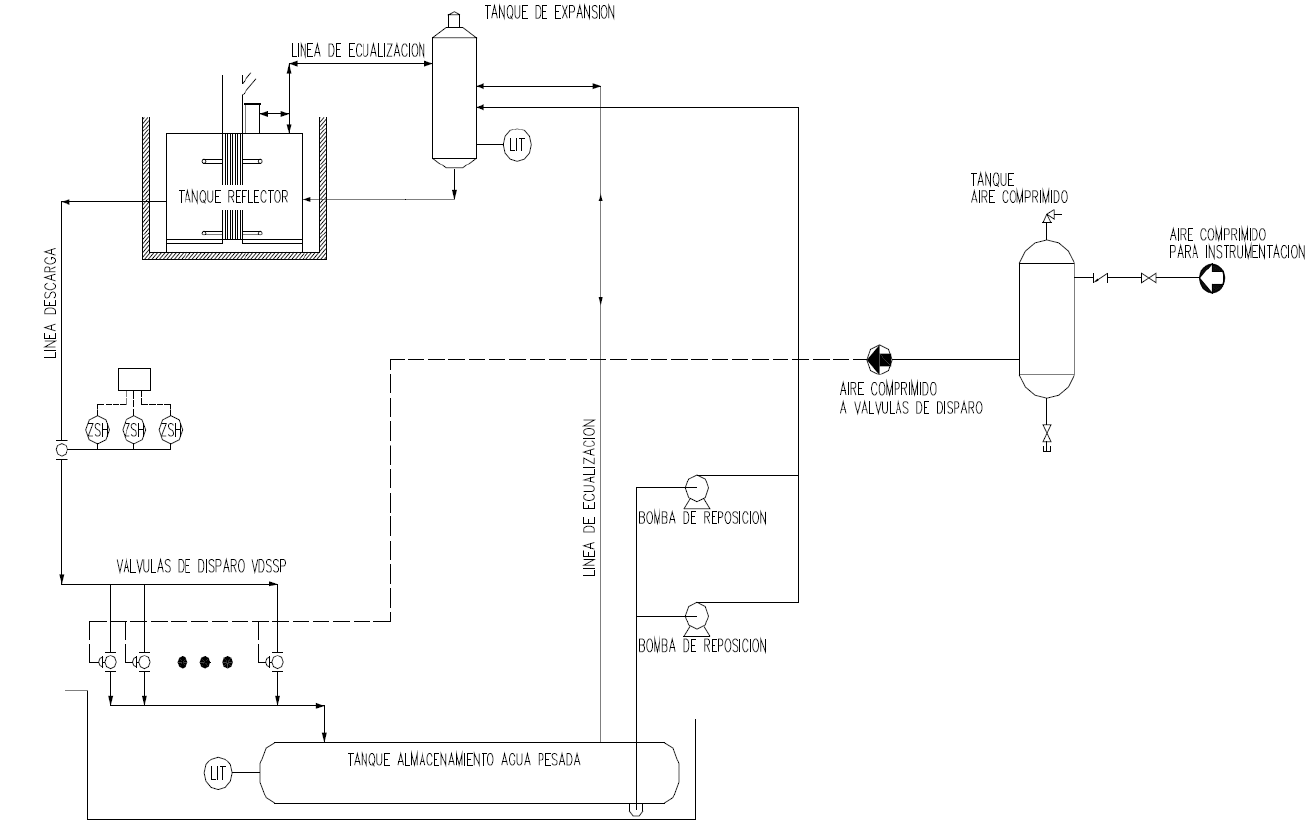
\includegraphics[scale=0.2]{ssp-mot.png}
      %~ \caption[]{t=250 s}
      %~ \label{ssp-mot}	
  %~ \end{minipage}
  %~ }

  \begin{figure}[ht]
    \begin{minipage}{0.4\linewidth}
      \centering
      %\includegraphics[scale=0.3]{cold-source-mot.png}
      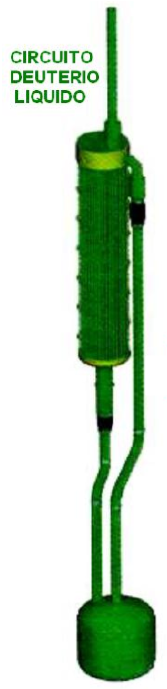
\includegraphics[scale=0.17]{deuterio.png}
      \caption[]{Esquema del circuito de deuterio en una fuente fría de neutrones.}
      \label{fuente-fria-mot}	
    \end{minipage}
    \begin{minipage}{0.58\linewidth}
      \centering
      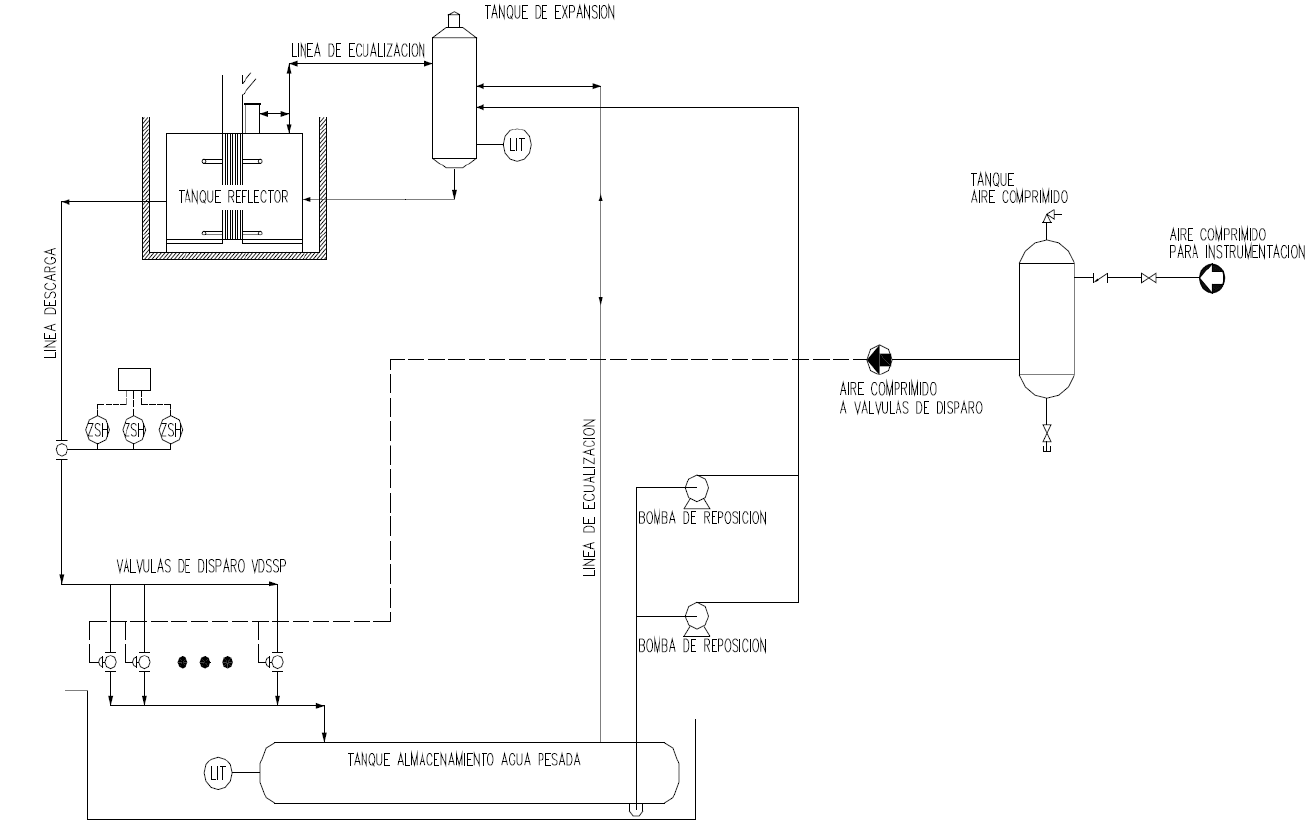
\includegraphics[scale=0.19]{ssp-mot.png}
      \caption[]{Esquema del Segundo Sistema de Parada del reactor RA-10.}
      \label{ssp-mot}	
    \end{minipage}
    %\caption[]{}  
    \label{aasdasd}
  \end{figure}
  
\end{frame}

\subsection{Abordaje del modelado}
\begin{frame}{Introducción}{Abordaje del modelado}


  \begin{figure}[ht]
%~ 
    \begin{minipage}{0.58\linewidth}
      \begin{itemize}
      \item <2-> Desglosar en subsistemas
      \item <3-> Identificar uniones que relacionan interfaces de acoplamiento
      \item <4-> Identificar pares de variables incógnitas en cada interfaz
      \item <5-> Total de incógnitas: 2N
        \begin{itemize}
        \item <6-> N ecuaciones de continuidad que relacionan las incógnitas entre dos interfaces contiguas de distintos subsistemas
        \item <7-> N ecuaciones modelos (acopladas) que relacionan las incógnitas (según selección de condiciones de borde)
        %\item <7-> N ecuaciones modelos que relacionan las incógnitas de la misma interfaz de cada subsistema
        \end{itemize} 
      \item <8-> Seleccionar método numérico y resolver
      \end{itemize}    
    \end{minipage}
%~ 
    \begin{minipage}{0.4\linewidth}
      \centering
      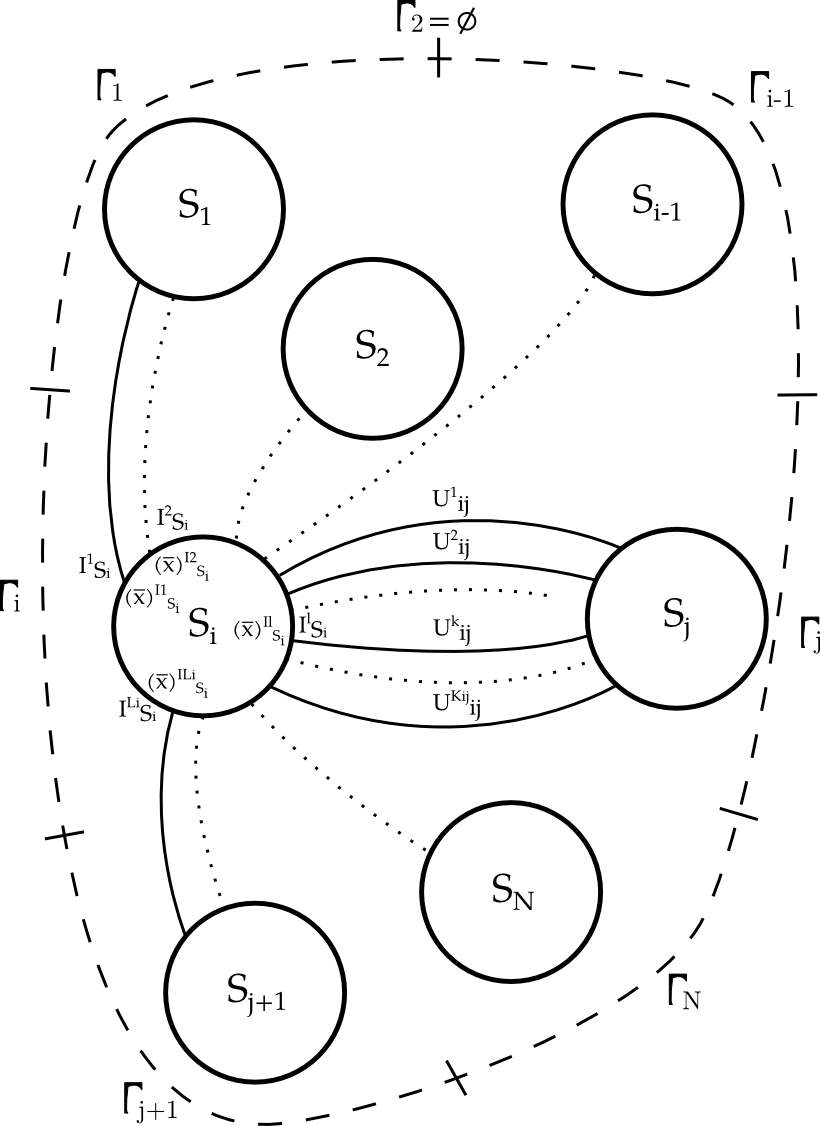
\includegraphics[scale=0.2]{coupling_systems.png}
      %\caption[]{Análisis de un sistema mediante el Método de Descomposición Disjunta de Dominios.}
      \label{esquma-DDM}
    \end{minipage}
        %~ 
    %\caption[]{}  
    \label{aasdasd}
  \end{figure}
  
  
\end{frame}



% You can reveal the parts of a slide one at a time
% with the \pause command:
\begin{frame}{Introducción}{Abordaje del modelado: Ejemplo}
Ejemplo: El dominio $\Omega$ representa una barra de largo $L$, coficiente de conductividad térmica $k$ y fuente interna de energía $f$.
Calcular el campo de temperaturas en $\Omega$ mediante el método
de Descomposición Disjunta de Dominios. Modelo:
\begin{equation*}
\left\{\begin{matrix}
-k \Delta u=f \\
\left.u\right|_{\partial\Omega}=0
\end{matrix}\right.
\label{ecuacion-calor}
\end{equation*}

\centering
%\raggedleft
  \begin{tikzpicture}[scale=0.750]
	\node at (12.5,4em) (om) {$\Omega$};

	\node at (7.5,5.9em) (Olabel) {0}; % 0
	\node at (7.5,5em) (O) {}; % point 0

	\node at (14.5,6.9em) (clabel) {c}; % c
	\node at (14.5,5em) (c) {}; % point c

	\node at (17.5,5.9em) (llabel) {L}; % L
	\node at (17.5,5em) (l) {}; % point L

	\draw[line width=1pt, o-|] (O) -- (c.center); % primer extremo de barra completa
	\draw[line width=1pt, |-o] (c.center) -- (l); % segundo extremo de barra completa
%~ 
	%~ \draw[line width=0.8pt,->] (11,3.5em) -- (10,1.5em); % primer flecha
	%~ \draw[line width=0.8pt,->] (16,3.5em) -- (17,1.5em); % segunda flecha
%~ 
	%~ \node at (10,-1em) (om1) {$\Omega_1$};
	%~ \node at (6.5,0.9em) (O1label) {0};
	%~ \node at (6.5,0em) (O1) {};
	%~ \node at (13.5,0.9em) (c1label) {c};
	%~ \node at (13.5,0em) (c1) {};
%~ 
	%~ \draw[line width=1pt, o-o] (O1) -- (c1); % primer barra
%~ 
	%~ \node at (17,-1em) (om2) {$\Omega_2$};
	%~ \node at (15.5,0.9em) (c2label) {c};
	%~ \node at (15.5,0em) (c2) {};
	%~ \node at (18.5,0.9em) (l2label) {L};
	%~ \node at (18.5,0em) (l2) {};
%~ 
	%~ \draw[line width=1pt, o-o] (c2) -- (l2); % segunda barra
  \end{tikzpicture}

\end{frame}


% You can reveal the parts of a slide one at a time
% with the \pause command:
\begin{frame}{Introducción}{Abordaje del modelado: Ejemplo}

\begin{itemize}
\item 1. Descomponer el dominio
\end{itemize}

\centering
%\raggedleft
  \begin{tikzpicture}[scale=0.750]
	\node at (12.5,4em) (om) {$\Omega$};

	\node at (7.5,5.9em) (Olabel) {0}; % 0
	\node at (7.5,5em) (O) {}; % point 0

	\node at (14.5,6.9em) (clabel) {c}; % c
	\node at (14.5,5em) (c) {}; % point c

	\node at (17.5,5.9em) (llabel) {L}; % L
	\node at (17.5,5em) (l) {}; % point L

	\draw[line width=1pt, o-|] (O) -- (c.center); % primer extremo de barra completa
	\draw[line width=1pt, |-o] (c.center) -- (l); % segundo extremo de barra completa

	\draw[line width=0.8pt,->] (11,3.5em) -- (10,1.5em); % primer flecha
	\draw[line width=0.8pt,->] (16,3.5em) -- (17,1.5em); % segunda flecha

	\node at (10,-1em) (om1) {$\Omega_1$};
	\node at (6.5,0.9em) (O1label) {0};
	\node at (6.5,0em) (O1) {};
	%~ \node at (13.5,0.9em) (c1label) {c};
	\node at (13.5,0em) (c1) {};

	\draw[line width=1pt, o-] (O1) -- (c1); % primer barra

	\node at (17,-1em) (om2) {$\Omega_2$};
	%~ \node at (15.5,0.9em) (c2label) {c};
	\node at (15.5,0em) (c2) {};
	\node at (18.5,0.9em) (l2label) {L};
	\node at (18.5,0em) (l2) {};

	\draw[line width=1pt, -o] (c2) -- (l2); % segunda barra
  \end{tikzpicture}

\end{frame}

% You can reveal the parts of a slide one at a time
% with the \pause command:
\begin{frame}{Introducción}{Abordaje del modelado: Ejemplo}

\begin{itemize}
\item 1. Descomponer el dominio
\item 2. Reconocer interfaces de acople
\end{itemize}

\centering
%\raggedleft
  \begin{tikzpicture}[scale=0.750]
	\node at (12.5,4em) (om) {$\Omega$};

	\node at (7.5,5.9em) (Olabel) {0}; % 0
	\node at (7.5,5em) (O) {}; % point 0

	\node at (14.5,6.9em) (clabel) {c}; % c
	\node at (14.5,5em) (c) {}; % point c

	\node at (17.5,5.9em) (llabel) {L}; % L
	\node at (17.5,5em) (l) {}; % point L

	\draw[line width=1pt, o-|] (O) -- (c.center); % primer extremo de barra completa
	\draw[line width=1pt, |-o] (c.center) -- (l); % segundo extremo de barra completa

	\draw[line width=0.8pt,->] (11,3.5em) -- (10,1.5em); % primer flecha
	\draw[line width=0.8pt,->] (16,3.5em) -- (17,1.5em); % segunda flecha

	\node at (10,-1em) (om1) {$\Omega_1$};
	\node at (6.5,0.9em) (O1label) {0};
	\node at (6.5,0em) (O1) {};
	\node at (13.5,0.9em) (c1label) {c};
	\node at (13.5,0em) (c1) {};

	\draw[line width=1pt, o-o] (O1) -- (c1); % primer barra

	\node at (17,-1em) (om2) {$\Omega_2$};
	\node at (15.5,0.9em) (c2label) {c};
	\node at (15.5,0em) (c2) {};
	\node at (18.5,0.9em) (l2label) {L};
	\node at (18.5,0em) (l2) {};

	\draw[line width=1pt, o-o] (c2) -- (l2); % segunda barra
  \end{tikzpicture}

\end{frame}

% You can reveal the parts of a slide one at a time
% with the \pause command:
\begin{frame}{Introducción}{Abordaje del modelado: Ejemplo}

\begin{itemize}
\item 1. Descomponer el dominio
\item 2. Reconocer interfaces de acople
\item 3. Identificar pares de variables de acoplamiento
\end{itemize}

\centering
%\raggedleft
  \begin{tikzpicture}[scale=0.750]%, every node/.style={scale=0.75}]
	\node at (12.5,4em) (om) {$\Omega$};

	\node at (7.5,5.9em) (Olabel) {0}; % 0
	\node at (7.5,5em) (O) {}; % point 0

	\node at (14.5,6.9em) (clabel) {c}; % c
	\node at (14.5,5em) (c) {}; % point c

	\node at (17.5,5.9em) (llabel) {L}; % L
	\node at (17.5,5em) (l) {}; % point L

	\draw[line width=1pt, o-|] (O) -- (c.center); % primer extremo de barra completa
	\draw[line width=1pt, |-o] (c.center) -- (l); % segundo extremo de barra completa

	\draw[line width=0.8pt,->] (11,3.5em) -- (10,1.5em); % primer flecha
	\draw[line width=0.8pt,->] (16,3.5em) -- (17,1.5em); % segunda flecha

	\node at (10,-1em) (om1) {$\Omega_1$};
	\node at (6.5,0.9em) (O1label) {0};
	\node at (6.5,0em) (O1) {};
	\node at (13.5,0.9em) (c1label) {c};
	\node at (13.2,-1.7em) (c1label) {\scriptsize $\{T_{S_1}, q''_{S_1}\}$};
	\node at (13.5,0em) (c1) {};

	\draw[line width=1pt, o-o] (O1) -- (c1); % primer barra

	\node at (17,-1em) (om2) {$\Omega_2$};
	\node at (15.5,0.9em) (c2label) {c};
  \node[align=center] at (15.7,-1.7em) (c1label) {\scriptsize $\{T_{S_2}, q''_{S_2}\}$};
	\node at (15.5,0em) (c2) {};
	\node at (18.5,0.9em) (l2label) {L};
	\node at (18.5,0em) (l2) {};

	\draw[line width=1pt, o-o] (c2) -- (l2); % segunda barra
  \end{tikzpicture}

\end{frame}

% You can reveal the parts of a slide one at a time
% with the \pause command:
\begin{frame}{Introducción}{Abordaje del modelado: Ejemplo}

%\centering
\raggedleft
  \begin{tikzpicture}[scale=0.50, every node/.style={scale=0.7}]
	\node at (12.5,4em) (om) {$\Omega$};

	\node at (7.5,5.9em) (Olabel) {0}; % 0
	\node at (7.5,5em) (O) {}; % point 0

	\node at (14.5,6.9em) (clabel) {c}; % c
	\node at (14.5,5em) (c) {}; % point c

	\node at (17.5,5.9em) (llabel) {L}; % L
	\node at (17.5,5em) (l) {}; % point L

	\draw[line width=1pt, o-|] (O) -- (c.center); % primer extremo de barra completa
	\draw[line width=1pt, |-o] (c.center) -- (l); % segundo extremo de barra completa

	\draw[line width=0.8pt,->] (11,3.5em) -- (10,1.5em); % primer flecha
	\draw[line width=0.8pt,->] (16,3.5em) -- (17,1.5em); % segunda flecha

	\node at (10,-1em) (om1) {$\Omega_1$};
	\node at (6.5,0.9em) (O1label) {0};
	\node at (6.5,0em) (O1) {};
	\node at (13.5,0.9em) (c1label) {c};
	\node at (13.2,-1.7em) (c1label) {\scriptsize $\{T_{S_1}, q''_{S_1}\}$};
	\node at (13.5,0em) (c1) {};

	\draw[line width=1pt, o-o] (O1) -- (c1); % primer barra

	\node at (17,-1em) (om2) {$\Omega_2$};
	\node at (15.5,0.9em) (c2label) {c};
  \node[align=center] at (15.7,-1.7em) (c1label) {\scriptsize $\{T_{S_2}, q''_{S_2}\}$};
	\node at (15.5,0em) (c2) {};
	\node at (18.5,0.9em) (l2label) {L};
	\node at (18.5,0em) (l2) {};

	\draw[line width=1pt, o-o] (c2) -- (l2); % segunda barra
  \end{tikzpicture}

\begin{itemize}
\item 4. Ecuaciones de continuidad: 
\begin{equation*}
\left\{\begin{matrix}
T_{S_1} = T_{S_2}=T \\
q''_{S_1} = q''_{S_2}=q''
\end{matrix}\right.
\end{equation*}
\end{itemize}

\end{frame}


% You can reveal the parts of a slide one at a time
% with the \pause command:
\begin{frame}{Introducción}{Abordaje del modelado: Ejemplo}

%\centering
\raggedleft
  \begin{tikzpicture}[scale=0.50, every node/.style={scale=0.7}]
	\node at (12.5,4em) (om) {$\Omega$};

	\node at (7.5,5.9em) (Olabel) {0}; % 0
	\node at (7.5,5em) (O) {}; % point 0

	\node at (14.5,6.9em) (clabel) {c}; % c
	\node at (14.5,5em) (c) {}; % point c

	\node at (17.5,5.9em) (llabel) {L}; % L
	\node at (17.5,5em) (l) {}; % point L

	\draw[line width=1pt, o-|] (O) -- (c.center); % primer extremo de barra completa
	\draw[line width=1pt, |-o] (c.center) -- (l); % segundo extremo de barra completa

	\draw[line width=0.8pt,->] (11,3.5em) -- (10,1.5em); % primer flecha
	\draw[line width=0.8pt,->] (16,3.5em) -- (17,1.5em); % segunda flecha

	\node at (10,-1em) (om1) {$\Omega_1$};
	\node at (6.5,0.9em) (O1label) {0};
	\node at (6.5,0em) (O1) {};
	\node at (13.5,0.9em) (c1label) {c};
	\node at (13.2,-1.7em) (c1label) {\scriptsize $\{T_{S_1}, q''_{S_1}\}$};
	\node at (13.5,0em) (c1) {};

	\draw[line width=1pt, o-o] (O1) -- (c1); % primer barra

	\node at (17,-1em) (om2) {$\Omega_2$};
	\node at (15.5,0.9em) (c2label) {c};
  \node[align=center] at (15.7,-1.7em) (c1label) {\scriptsize $\{T_{S_2}, q''_{S_2}\}$};
	\node at (15.5,0em) (c2) {};
	\node at (18.5,0.9em) (l2label) {L};
	\node at (18.5,0em) (l2) {};

	\draw[line width=1pt, o-o] (c2) -- (l2); % segunda barra
  \end{tikzpicture}

\begin{itemize}
\item 5. Ecuaciones modelos según condiciones de borde: 
  \begin{itemize}
  \item a. Selección de condiciones de borde:
    \begin{itemize}
    \item $S_1$ condición de tipo $Dirichlet$ (recibe $T^{guess}$)
    \item $S_2$ condición de tipo $Neumann$ (recibe $q''^{guess}$)
    \end{itemize}
  \item b. Selección de ecuaciones modelos:
  \begin{equation*}
  \left\{\begin{matrix}
  (q''^{calc})_{S_1} = \mathscr{N}_1\left ((T^{guess})_{S_1}\right ) \\
  (T^{calc})_{S_2} = \mathscr{D}_2\left ((q''^{guess})_{S_2}\right )
  \end{matrix}\right.
  \end{equation*}
  \end{itemize}
\end{itemize}

\end{frame}


% You can reveal the parts of a slide one at a time
% with the \pause command:
\begin{frame}{Introducción}{Abordaje del modelado: Ejemplo}

%\centering
\raggedleft
  \begin{tikzpicture}[scale=0.50, every node/.style={scale=0.7}]
	\node at (12.5,4em) (om) {$\Omega$};

	\node at (7.5,5.9em) (Olabel) {0}; % 0
	\node at (7.5,5em) (O) {}; % point 0

	\node at (14.5,6.9em) (clabel) {c}; % c
	\node at (14.5,5em) (c) {}; % point c

	\node at (17.5,5.9em) (llabel) {L}; % L
	\node at (17.5,5em) (l) {}; % point L

	\draw[line width=1pt, o-|] (O) -- (c.center); % primer extremo de barra completa
	\draw[line width=1pt, |-o] (c.center) -- (l); % segundo extremo de barra completa

	\draw[line width=0.8pt,->] (11,3.5em) -- (10,1.5em); % primer flecha
	\draw[line width=0.8pt,->] (16,3.5em) -- (17,1.5em); % segunda flecha

	\node at (10,-1em) (om1) {$\Omega_1$};
	\node at (6.5,0.9em) (O1label) {0};
	\node at (6.5,0em) (O1) {};
	\node at (13.5,0.9em) (c1label) {c};
	\node at (13.2,-1.7em) (c1label) {\scriptsize $\{T_{S_1}, q''_{S_1}\}$};
	\node at (13.5,0em) (c1) {};

	\draw[line width=1pt, o-o] (O1) -- (c1); % primer barra

	\node at (17,-1em) (om2) {$\Omega_2$};
	\node at (15.5,0.9em) (c2label) {c};
  \node[align=center] at (15.7,-1.7em) (c1label) {\scriptsize $\{T_{S_2}, q''_{S_2}\}$};
	\node at (15.5,0em) (c2) {};
	\node at (18.5,0.9em) (l2label) {L};
	\node at (18.5,0em) (l2) {};

	\draw[line width=1pt, o-o] (c2) -- (l2); % segunda barra
  \end{tikzpicture}

\begin{itemize}
\item 6. Seleccionar método numérico y resolver: 
  \begin{itemize}
  \item a. Métodos explícitos:
    \begin{itemize}
    \item a1. $Dirichlet-to-Neumann$ (cálculos en serie):
      \begin{equation*}
      \left\{\begin{matrix}
      (q''^{calc})_{S_1} = \mathscr{N}_1\left ((T^{guess})_{S_1}\right ) \\
      (T^{calc})_{S_2} = \mathscr{D}_2\left ((q''^{calc})_{S_1}\right )
      \end{matrix}\right.
      \end{equation*}
    \end{itemize}
  \end{itemize}
\end{itemize}

\end{frame}

% You can reveal the parts of a slide one at a time
% with the \pause command:
\begin{frame}{Introducción}{Abordaje del modelado: Ejemplo}

%\centering
\raggedleft
  \begin{tikzpicture}[scale=0.50, every node/.style={scale=0.7}]
	\node at (12.5,4em) (om) {$\Omega$};

	\node at (7.5,5.9em) (Olabel) {0}; % 0
	\node at (7.5,5em) (O) {}; % point 0

	\node at (14.5,6.9em) (clabel) {c}; % c
	\node at (14.5,5em) (c) {}; % point c

	\node at (17.5,5.9em) (llabel) {L}; % L
	\node at (17.5,5em) (l) {}; % point L

	\draw[line width=1pt, o-|] (O) -- (c.center); % primer extremo de barra completa
	\draw[line width=1pt, |-o] (c.center) -- (l); % segundo extremo de barra completa

	\draw[line width=0.8pt,->] (11,3.5em) -- (10,1.5em); % primer flecha
	\draw[line width=0.8pt,->] (16,3.5em) -- (17,1.5em); % segunda flecha

	\node at (10,-1em) (om1) {$\Omega_1$};
	\node at (6.5,0.9em) (O1label) {0};
	\node at (6.5,0em) (O1) {};
	\node at (13.5,0.9em) (c1label) {c};
	\node at (13.2,-1.7em) (c1label) {\scriptsize $\{T_{S_1}, q''_{S_1}\}$};
	\node at (13.5,0em) (c1) {};

	\draw[line width=1pt, o-o] (O1) -- (c1); % primer barra

	\node at (17,-1em) (om2) {$\Omega_2$};
	\node at (15.5,0.9em) (c2label) {c};
  \node[align=center] at (15.7,-1.7em) (c1label) {\scriptsize $\{T_{S_2}, q''_{S_2}\}$};
	\node at (15.5,0em) (c2) {};
	\node at (18.5,0.9em) (l2label) {L};
	\node at (18.5,0em) (l2) {};

	\draw[line width=1pt, o-o] (c2) -- (l2); % segunda barra
  \end{tikzpicture}

\begin{itemize}
\item 6. Seleccionar método numérico y resolver: 
  \begin{itemize}
  \item a. Métodos explícitos:
    \begin{itemize}
    \item a2. $Punto$ $fijo$ (cálculos en paralelo):
      \begin{equation*}
      \left\{\begin{matrix}
      (q''^{calc})_{S_1} = \mathscr{N}_1\left ((T^{guess})_{S_1}\right ) \\
      (T^{calc})_{S_2} = \mathscr{D}_2\left ((q''^{guess})_{S_2}\right )
      \end{matrix}\right.
      \end{equation*}
    \end{itemize}
  \end{itemize}
\end{itemize}

\end{frame}


\begin{frame}{Introducción}{Abordaje del modelado: Ejemplo}

%\centering
\raggedleft
  \begin{tikzpicture}[scale=0.50, every node/.style={scale=0.7}]
	\node at (12.5,4em) (om) {$\Omega$};

	\node at (7.5,5.9em) (Olabel) {0}; % 0
	\node at (7.5,5em) (O) {}; % point 0

	\node at (14.5,6.9em) (clabel) {c}; % c
	\node at (14.5,5em) (c) {}; % point c

	\node at (17.5,5.9em) (llabel) {L}; % L
	\node at (17.5,5em) (l) {}; % point L

	\draw[line width=1pt, o-|] (O) -- (c.center); % primer extremo de barra completa
	\draw[line width=1pt, |-o] (c.center) -- (l); % segundo extremo de barra completa

	\draw[line width=0.8pt,->] (11,3.5em) -- (10,1.5em); % primer flecha
	\draw[line width=0.8pt,->] (16,3.5em) -- (17,1.5em); % segunda flecha

	\node at (10,-1em) (om1) {$\Omega_1$};
	\node at (6.5,0.9em) (O1label) {0};
	\node at (6.5,0em) (O1) {};
	\node at (13.5,0.9em) (c1label) {c};
	\node at (13.2,-1.7em) (c1label) {\scriptsize $\{T_{S_1}, q''_{S_1}\}$};
	\node at (13.5,0em) (c1) {};

	\draw[line width=1pt, o-o] (O1) -- (c1); % primer barra

	\node at (17,-1em) (om2) {$\Omega_2$};
	\node at (15.5,0.9em) (c2label) {c};
  \node[align=center] at (15.7,-1.7em) (c1label) {\scriptsize $\{T_{S_2}, q''_{S_2}\}$};
	\node at (15.5,0em) (c2) {};
	\node at (18.5,0.9em) (l2label) {L};
	\node at (18.5,0em) (l2) {};

	\draw[line width=1pt, o-o] (c2) -- (l2); % segunda barra
  \end{tikzpicture}

\begin{itemize}
\item 6. Seleccionar método numérico y resolver: 
  \begin{itemize}
  \item a. Métodos implícitos (cálculos en paralelo):
  Búsqueda de raíces de las ecuaciones de residuos:
  \begin{equation*}
  \left\{\begin{matrix}
  (r_{q''})_{S_1}^{1}  = (q''^{ guess}) - (q''^{calc})_{S_1} \\
  (r_{q''})_{S_2}^{1}  = (T^{guess}) - (T^{calc})_{S_2}
  \end{matrix}\right.
  \label{res_qt}
  \end{equation*}
    \begin{itemize}
    \item a1. $Newton-Raphson$
    \item a2. $Quasi-Newton$
    \item a3. $Newton-Krylov$
    \end{itemize}
  \end{itemize}
\end{itemize}

\end{frame}

\begin{frame}{Introducción}{Abordaje del modelado}

Algunos métodos requieren construcción de matriz jacobiana.

Cada elemento $J_{ij}=\frac{\partial R_i}{\partial x_j}$ puede aproximarse mediante diferencias finitas a primer orden como:

\begin{equation*}
J_{ij} \approx \frac{r_i(\bar{x} + \Delta \bar{x}^j) - r_i(\bar{x})}{\left\|\Delta \bar{x}^j\right\|}
\label{j-diff}
\end{equation*}
donde $\Delta \bar{x}^j=\bar{\epsilon}^j \cdot \Delta^j$

\end{frame}

\begin{frame}{Introducción}{Abordaje del modelado}
  \centering
  \captionof{table}{Principales características de los métodos utilizados}\label{table:metodos}
  \resizebox{\linewidth}{!}{
  \begin{tabular}{lll}
  \hline
  \textbf{}                                        & Métodos explícitos                         & Métodos implícitos                             \\ \hline \hline
  Ventajas                                         & Fácil implementación                       & Implementación compleja                        \\
  \multicolumn{1}{c}{\multirow{2}{*}{Desventajas}} & Selección de condiciones de borde limitada & Libertad en selección de condiciones de borde  \\
  \multicolumn{1}{c}{}                             & En general convergencia más lenta          & En general mejores propiedades de convergencia \\ \hline
  \end{tabular}
  }
\end{frame}


\begin{frame}{Introducción}{Problemas de evolución}

Estrategia:
\begin{itemize}
\item <2-> Cada susistema utiliza su propia discretización temporal.
\item <3-> La discretización debe coincidir al comienzo (condiciones iniciales), al final y en puntos a lo largo de la evolución.
\item <4-> Los resultados se acoplan en estos puntos de coincidencia. 
\item <5-> Usando métodos iterativos, cada iteración comienza la resolución desde el último punto acoplado (en el que convergieron los resultados).
\item <6-> Esta metodología no altera las propiedades de estabilidad temporal del método numérico particular utilizado para resolver cada subsistema.
\end{itemize}

\centering

  \begin{tikzpicture}%[scale=0.50, every node/.style={scale=0.7}]

	\node at (-12em,0em) (c11) {$S_1$};
	\node at (-12em,-2em) (c11) {$S_2$};
  
	\node at (-10em,0em) (c11) {\scriptsize $t_0$};
	\node at (-10em,-2em) (c21) {\scriptsize $t_0$};

  \node at (-5em,0em) (c12) {};
	\node at (-5em,-2em) (c22) {};
  
    
  \node at (0em,0em) (c13) {};
	\node at (0em,-2em) (c23) {};
  
  \node at (5em,0em) (c14) {};
	\node at (5em,-2em) (c24) {};

  \node at (10em,0em) (c15) {\scriptsize $t_f$};
	\node at (10em,-2em) (c25) {\scriptsize $t_f$};  
  
  
	\draw[line width=1pt, |-|] (c11) -- (c12.center);
	\draw[line width=1pt, |-|] (c12.center) -- (c13.center);
	\draw[line width=1pt, |-|] (c13.center) -- (c14.center);
	\draw[line width=1pt, |-|] (c14.center) -- (c15);
	\draw[line width=1pt, |-|] (c21) -- node[midway]{$|$} (c22.center);
	\draw[line width=1pt, |-|] (c22.center) -- node[midway]{$|$} (c23.center);
	\draw[line width=1pt, |-|] (c23.center) -- node[midway]{$|$} (c24.center);
	\draw[line width=1pt, |-|] (c24.center) -- node[midway]{$|$}  (c25);

	
  \end{tikzpicture}

\end{frame}

\subsection{Objetivos}

\begin{frame}{Introducción}{Objetivos}

Considerando la motivación y la formulación precedente, queda establecido el siguiente objetivo general de la maestría:
\vspace{1em}

\textit{Desarrollar una estrategia de resolución de problemas complejos formulados mediante el
Método de Descomposición Disjunta de Dominios que permita resolver subproblemas separados con códigos de cálculo específicos,
manteniendo la interacción entre ellos solo mediante condiciones de borde.}

\end{frame}
 % intro
\section{Estrategia de resolución}% mediante acoplamiento de códigos}

\subsection{Paradigma maestro-esclavo}

\begin{frame}
{Estrategia de resolución mediante acoplamiento de códigos}
{Paradigma maestro-esclavo}
%~ 
%~ \begin{figure}
\centering
\begin{tikzpicture}[
  scale=0.7, every node/.style={scale=0.7},
	block1/.style={
	draw,
	fill=white,
	rectangle, 
	%~ minimum width={width("Proceso $N_m$")+2pt},
	%~ minimum height={15pt},
	font=\small},
	block2/.style={
	draw,
	%~ fill=white,
	rectangle,
  fill=blue!20,
  text centered, 
  rounded corners,
	%~ minimum width={width("Esclavo N")+2pt},
	%~ minimum height={15pt},
	font=\large},
	connector/.style={
	-o,
	line width=0.3mm
	},
  arrow1/.style={
  -{Latex[length=3mm, width=1mm]}
  },
  arrow2/.style={
  {Latex[length=3mm, width=1mm]}-{Latex[length=3mm, width=1mm]}
  }]

	% Dummy
	\node at (0,10em)             (dummy) {}; % blank space

	% Master
	\node [draw,fill=blue!20,text centered,rounded corners] at (0,8em)             (master) {\textbf{Maestro}};
	\node [block2] at (0,8em)             (master) {\textbf{Maestro}};
	\node [block1, below=1em of master]   (masterp1) {...};
	\node [block1, left=1em of masterp1]  (masterp0) {Proceso $0_m$};	
	\node [block1, right=1em of masterp1] (masterpN) {Proceso $N_m$};

	% Slave 1
	\node [block2] at (-6.5,0em)    		(slave1) {\textbf{Esclavo 1}};
	\node [block1, below=1em of slave1] (s1p0) 	 {Proceso $0_1$};
	\node [block1, below=1em of s1p0]   (s1p1) 	 {...};
	\node [block1, below=1em of s1p1] 	(s1pN) 	 {Proceso $N_1$};
	%~ 
	% Slave 2
	\node [block2] at (-3.5,-4em)    		(slave2) {\textbf{Esclavo 2}};
	\node [block1, below=1em of slave2] (s2p0) 	 {Proceso $0_2$};
	\node [block1, below=1em of s2p0]   (s2p1) 	 {...};
	\node [block1, below=1em of s2p1] 	(s2pN) 	 {Proceso $N_2$};
	
	% Slave 3
	\node [block2] at (0,0em)      		  (slave3) {\textbf{Esclavo 3}};
	\node [block1, below=1em of slave3] (s3p0) 	 {Proceso $0_3$};
	\node [block1, below=1em of s3p0]   (s3p1) 	 {...};
	\node [block1, below=1em of s3p1] 	(s3pN) 	 {Proceso $N_3$};
	
	% Slave 4
	\node [block2] at (3.5,-4em)   		  (slave4) {\textbf{Esclavo $i$}};
	\node [block1, below=1em of slave4] (s4p0) 	 {Proceso $0_i$};
	\node [block1, below=1em of s4p0]   (s4p1) 	 {...};
	\node [block1, below=1em of s4p1] 	(s4pN) 	 {Proceso $N_i$};
	
	% Slave N
	\node [block2] at (6.5,0em)    		  (slave5) {\textbf{Esclavo N}};
	\node [block1, below=1em of slave5] (s5p0) 	 {Proceso $0_N$};

	% Processes
	\draw[connector] (master.south) -- ($(masterp0.north)+(0,0.2em)$);
	\draw[connector] (master.south) -- ($(masterp1.north)+(0,0em)$);
	\draw[connector] (master.south) -- ($(masterpN.north)+(0,0.2em)$);

	\draw[connector] (slave1.west) -- ++(-1em,0) |- (s1p0.west);
	\draw[connector] (slave1.west) -- ++(-1em,0) |- (s1p1.west);
	\draw[connector] (slave1.west) -- ++(-1em,0) |- (s1pN.west);

	\draw[connector] (slave2.west) -- ++(-1em,0) |- (s2p0.west);
	\draw[connector] (slave2.west) -- ++(-1em,0) |- (s2p1.west);
	\draw[connector] (slave2.west) -- ++(-1em,0) |- (s2pN.west);

	\draw[connector] (slave3.west) -- ++(-1em,0) |- (s3p0.west);
	\draw[connector] (slave3.west) -- ++(-1em,0) |- (s3p1.west);
	\draw[connector] (slave3.west) -- ++(-1em,0) |- (s3pN.west);

	\draw[connector] (slave4.west) -- ++(-1em,0) |- (s4p0.west);
	\draw[connector] (slave4.west) -- ++(-1em,0) |- (s4p1.west);
	\draw[connector] (slave4.west) -- ++(-1em,0) |- (s4pN.west);

	\draw[connector] (slave5.west) -- ++(-1em,0) |- (s5p0.west);


	% Comunicators
	\draw[arrow2] ($(masterp0.south)-(1em,0)$) to[out=-90, in=15, distance=2em] node [midway, sloped, anchor=center, above]{\textit{MPI}} (s1p0.east);

	\draw[arrow2] ($(masterp0.south)+(0em,0)$) to[out=-90, in=35, distance=3em] node [midway, rotate=90, anchor=center, above]{\textit{MPI}} (s2p0.east);

	\draw[arrow1] ($(masterp0.south)+(1em,0)$) to[out=-90, in=105, distance=2em] node [midway, sloped, anchor=center, above]{\textit{I/O}} (slave3.north);

	\draw[arrow1] (masterp1.south) to[out=-90, in=105, distance=2em] node [midway, sloped, anchor=center, above]{\textit{I/O}} (slave4.north);

	\draw[arrow1] (masterpN.south) to[out=-90, in=105, distance=2em] node [midway, sloped, anchor=center, above]{\textit{I/O}} (slave5.north);

\end{tikzpicture}
%~ \caption[Esquema de comunicación entre programas implementado]{Esquema de comunicación entre los programas \textit{esclavos} y el programa \textit{maestro} implementado en el acoplamiento de códigos.
%~ Los \textit{esclavos} se comunican solo con el \textit{maestro} y no intercambian datos entre sí.
%~ Se utilizan dos modelos de comunicación diferentes.
%~ En el primero, cada código \textit{esclavo} es comunicado con el código \textit{maestro} a por paso de mensajes (indicado como \textit{MPI}).
%~ Como podrían correr en modo serial o paralelo, solo sus procesos \textit{raíces} establecen la comunicación con el proceso \textit{raíz} del programa \textit{maestro}.
%~ En el segundo modelo de comunicación, los códigos \textit{esclavos} son directamente \textit{ejecutados} por el programa \textit{maestro} en uno o varios procesos.
%~ En este modelo, la comunicación se establece solo mediante lectura y escritura de archivos (indicado como \textit{I/O}).}
%~ \label{esquema-comunicacion}
%~ \end{figure}

\end{frame}


\subsection{Modelos de comunicación}

\begin{frame}
{Estrategia de resolución mediante acoplamiento de códigos}
{Modelos de comunicación}

\begin{itemize}
\item <1-> Paso de mensajes: este modelo es implementado para comunicar procesos de programas en los cuales es posible modificar sus códigos fuente.
  \begin{itemize}
  \item Programas ejecutados en forma independiente y conectados
  \item Programas ejecutados en simultáneo como argumentos de $mpirun$
  \end{itemize}
\item <2-> Escritura de archivos de entrada y lectura de archivos de salida: este modelo es implementado para comunicar procesos de programas en los cuales NO es posible modificar sus códigos fuente.
\end{itemize}

\end{frame}


\subsection{Arquitectura de acoplamiento montada en códigos esclavos comunicados por paso de mensajes}

\begin{frame}
{Estrategia de resolución mediante acoplamiento de códigos}
{Arquitectura de acoplamiento montada en códigos esclavos comunicados por paso de mensajes}

\begin{figure}
\centering{}
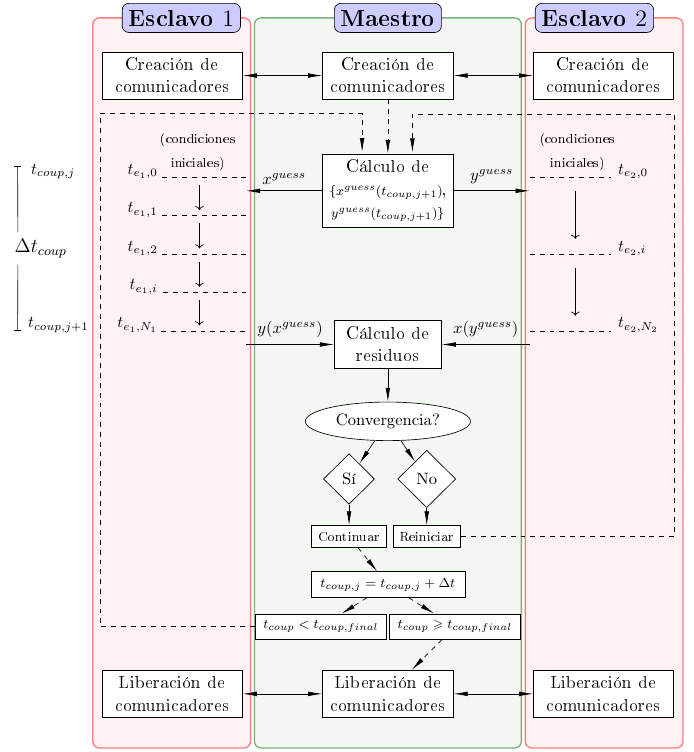
\includegraphics[scale=0.27]{esquema-acoplamiento.png}
\end{figure}


\end{frame}

\subsection{Códigos maestro utilizados}

\begin{frame}
{Estrategia de resolución mediante acoplamiento de códigos}
{Códigos maestro utilizados}

\begin{itemize}
\item \textbf{Coupling} \cite{coup-0d3d} \cite{coup-black} \cite{coup-hyd}
  \begin{itemize}
  \item <1-> Modelos de comunicación por paso de mensajes entre programas ejecutados de manera independiente
  \item <2-> Cada interfaz de acople tiene $N$ pares de variables incógnitas
  \item <3-> Métodos de resolución explícitos e implícitos implementados
  \end{itemize}
\end{itemize}

\end{frame}

\begin{frame}
{Estrategia de resolución mediante acoplamiento de códigos}
{Códigos maestro utilizados}

\begin{itemize}
\item \textbf{Newton} (desarrollado durante la maestría)
  \begin{itemize}
  \item <1-> Modelos de comunicación por paso de mensajes entre programas ejecutados de manera independiente o simultánea
  \item <2-> Modelos de comunicación por manejo de archivos
  \item <3-> Cada subsistema tiene $N$ incógnitas (extensión a acoplamientos genéricos)
  \item <4-> Métodos de resolución explícitos e implícitos implementados
  \item <5-> Mapeos de variables de entrada y salida ($\alpha-\beta$ y $\gamma-\delta$)
  \end{itemize}
\end{itemize}

%~ \begin{figure}
\centering{}
\visible <5>{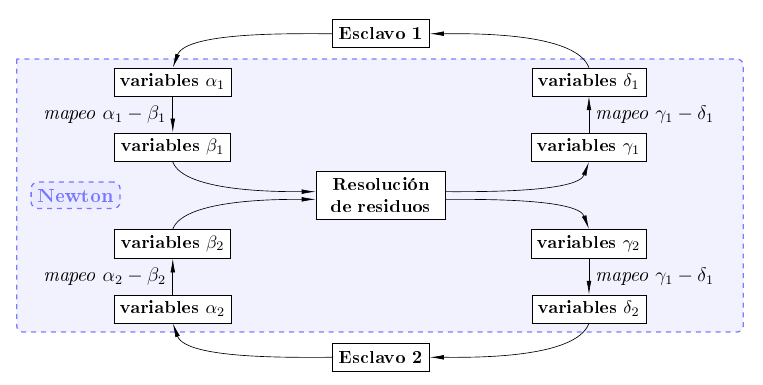
\includegraphics[scale=0.4]{abgd.png}}
%~ \end{figure}

\end{frame}
 % códigos
\section{Ejemplos de aplicación}

\subsection{Movimiento por fuerza boyante en un circuito cerrado}

\begin{frame}
{Ejemplos de aplicación}
{Fluidodinámica en una fuente fría de neutrones}

\begin{figure}
\centering{}
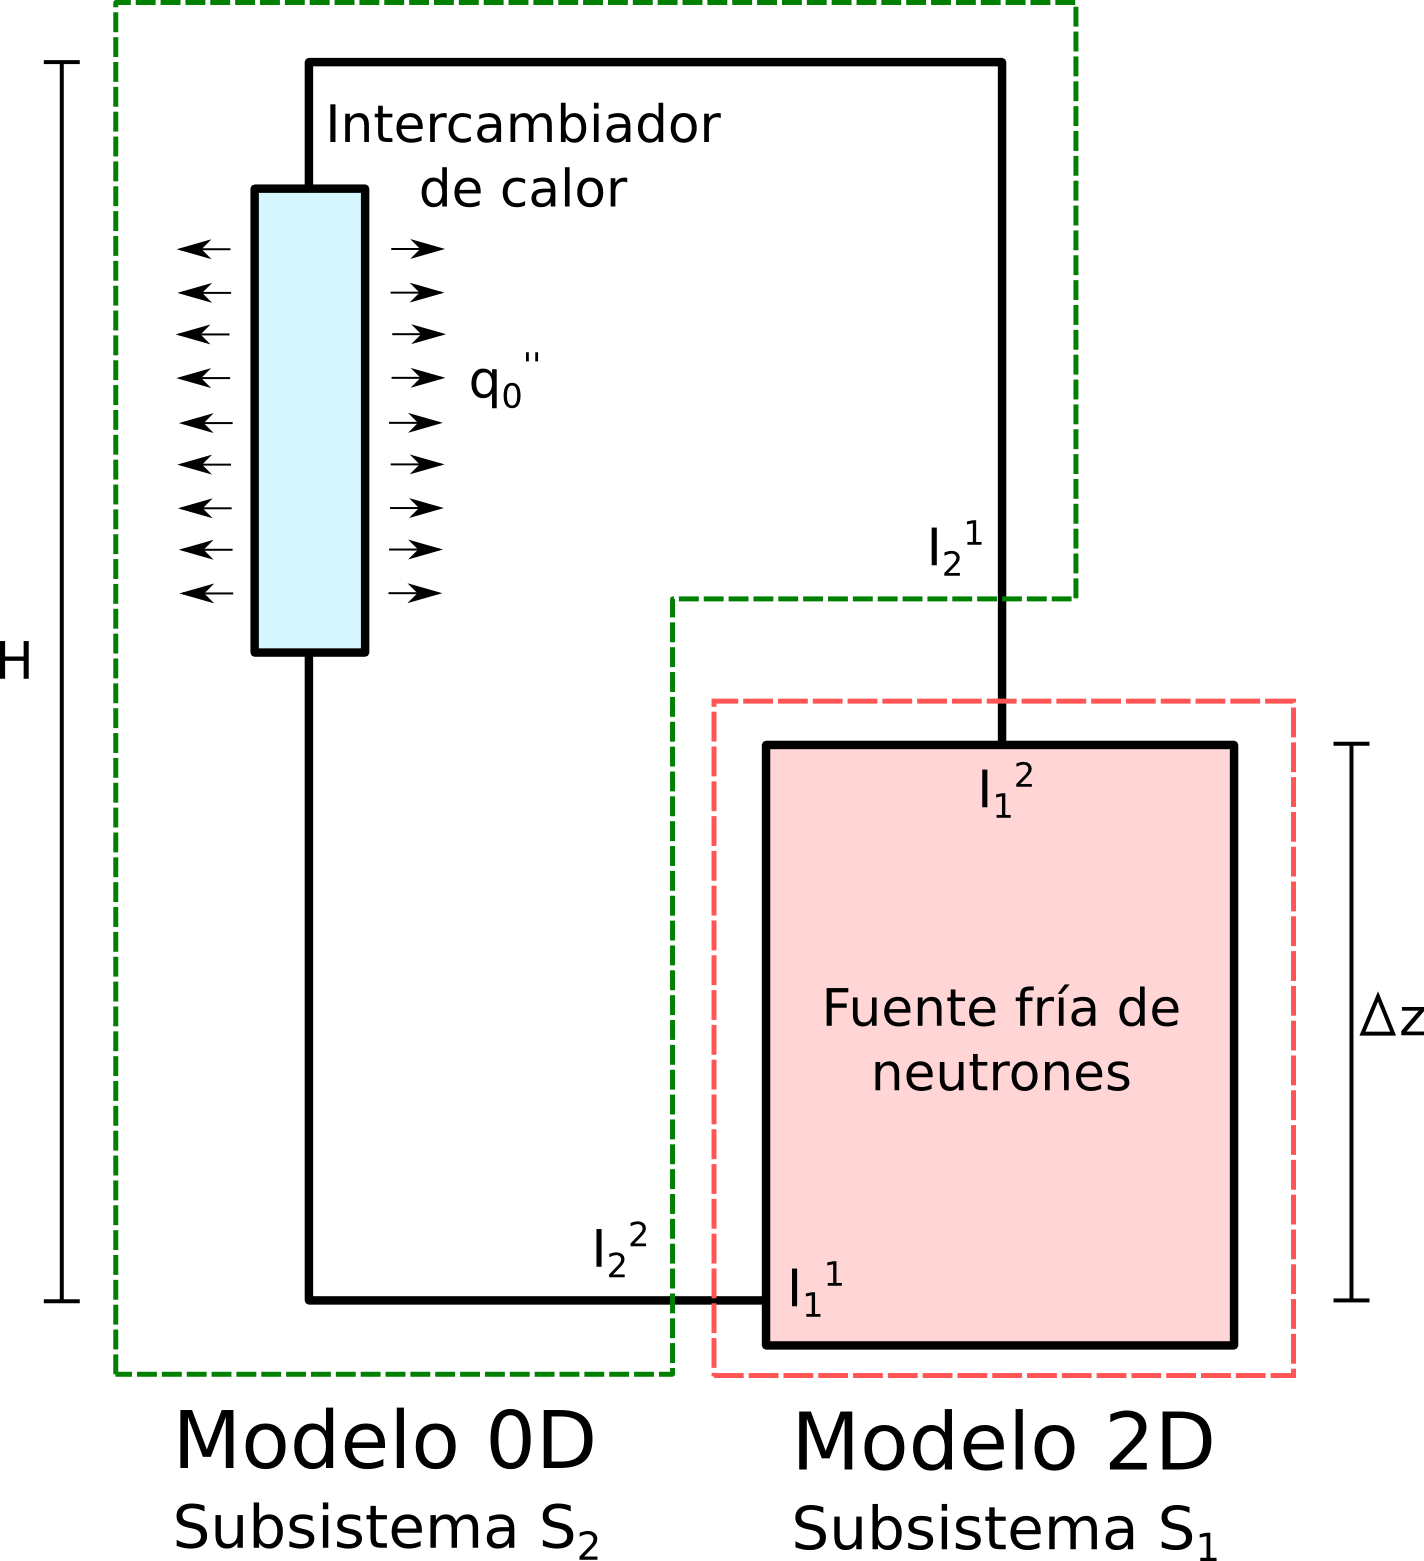
\includegraphics[scale=0.27]{fuente-fria.png}
\end{figure}

\end{frame}

\begin{frame}
{Ejemplos de aplicación}
{Fluidodinámica en una fuente fría de neutrones}

Sistema $S_1$:

\visible<2->{
Parámetros utilizados: $\rho_0=163$ $Kg/m^3$ a la temperatura de referencia $T_{ref}$,
$\mu=2.8\cdot 10^{-5}$ $Kg/ms$, $c_p=6333.6$ $J/KgK$, 
$k=0.136$ $W/mK$ y $\beta=1.32\cdot10^{-2}K^{-1}$.
Las áreas de las interfaces de acople son $A_2^1=A_2^2=0.03$ $m^2$.
}

\visible <3>{
\begin{equation*}
\left\{ \begin{array}{lr}
\displaystyle \frac {\partial \bar{u}}{\partial t} + ( \bar{u} \cdot \nabla) \bar{u} = - \frac {\nabla p}{\rho_0}
+ \left( 1- \beta (T-T_{ref}) \right)\bar{g} + \\ [0.24cm]
+ \nabla \cdot \left[ \left( \nu\right) \left( \nabla \bar{u} + \nabla \bar{u}^T \right) \right] \\ [0.2cm]
\nabla \cdot \bar{u} = 0 \\ [0.2cm]
\displaystyle \frac {\partial T}{\partial t} + ( \bar{u} \cdot \nabla) T = \frac {k}{\rho_0 c_p} \Delta T + \frac{f_0}{\rho_0 c_p}
\label{eq-cavidad}
\end{array}
\right.
\end{equation*}
donde $\bar{u}$ es el campo de velocidades dentro de la cavidad,
$p$ el campo de presiones y
$T$ el campo de temperaturas.
}

\end{frame}

\begin{frame}
{Ejemplos de aplicación}
{Fluidodinámica en una fuente fría de neutrones}

Sistema $S_2$:

\visible<2->{
Parámetros extra utilizados:
longitud total de cañerías $L=15$ $m$, 
sumatoria de coeficientes de pérdida de carga concentrada $\sum K_i=1.72$, 
rugosidad de cañerías $\epsilon=0.5\cdot 10^{-4}$ $m$.
}

\visible <3>{
\begin{equation*}
\left\{ \begin{array}{l}
Q_2^{2} = Q_2^{1} \\ [0.2cm]
p_2^2 = p_2^1 + \rho_0 g \left ( \Delta z + \beta (T_2^1 - T_{ref}) (H-\Delta z) \right ) - \\ [0.2cm]
- \rho_0 \frac{1}{2} \left( \frac{Q_1^1}{A_2^1} \right)^2  \left( \frac {f_D L} {D} + \sum_i K_i \right)  \\ [0.2cm]
T_2^2 = 0
%T_2^2 =& T_2^1 + 2 \frac {q_0" L}{\frac{D}{2} \frac{Q_1^1}{A_2^1}\rho c_p}
\label{eq-intercambiador}
\end{array}
\right.
\end{equation*}
donde $Q_2^i$ es el caudal en la interfaz $i$,
$p_2^i$ es la presión del subsistema promediada en esta interfaz,
$T_2^i$ es la temperatura promediada en esta interfaz,
$g$ es la aceleración generada por el campo gravitatorio,
$f_D$ es el factor de $Darcy$ de pérdida de carga distribuida,
y $D$ es el diámetro de la tubería.
}
\end{frame}

\begin{frame}
{Ejemplos de aplicación}
{Fluidodinámica en una fuente fría de neutrones}

Estrategia de resolución:

\begin{itemize}
\item Ecuaciones de continuidad
\begin{equation*}
\left\{ \begin{array}{l}
Q_1^1= Q_2^2 \\
Q_1^2= Q_2^1 \\
p_1^1= p_2^2 \\
p_1^2= p_2^1 \\
T_2^1= T_2^2 \\
T_2^2= T_2^1 \\
q"_2^1= - q"_2^2 \\
q"_2^2= - q"_2^1
\end{array}
\right.
\end{equation*}
\end{itemize}

\end{frame}

\begin{frame}
{Ejemplos de aplicación}
{Fluidodinámica en una fuente fría de neutrones}

\begin{itemize}
\item Selección de condiciones de borde
  \begin{itemize}
  \item en la interfaz inferior de la cavidad 2-D:
      \begin{itemize}
      \item condiciones de tipo \textit{Dirichlet} para el par presión-caudal
      \item condiciones de tipo \textit{Dirichlet} para el par temperatura-flujo de calor
      \end{itemize}
  \item en la interfaz superior de la cavidad 2-D:
      \begin{itemize}
      \item condiciones de tipo \textit{Neumann} para el par presión-caudal
      \item condiciones de tipo \textit{Neumann} para el par temperatura-flujo de calor
      \end{itemize}
  \visible<2>{\item en la interfaz inferior de la red 0-D:
      \begin{itemize}
      \item condiciones de tipo \textit{Neumann} para el par presión-caudal
      \item condiciones de tipo \textit{Neumann} para el par temperatura-flujo de calor
      \end{itemize}
  \item en la interfaz superior de la red 0-D:
      \begin{itemize}
      \item condiciones de tipo \textit{Neumann} para el par presión-caudal
      \item condiciones de tipo \textit{Dirichlet} para el par temperatura-flujo de calor
      \end{itemize}}
  \end{itemize} 

\end{itemize}

\end{frame}



\begin{frame}
{Ejemplos de aplicación}
{Fluidodinámica en una fuente fría de neutrones}

\begin{itemize}
\item Ecuaciones de residuos en subsistema 1:

\begin{equation*}
\left\{ \begin{array}{l}
(R_{p,Q})_{1}^{1}  = p_1^{1, guess} - p_1^{1, calc}(Q_1^{1, guess}, T_1^{1, guess}, p_1^{2, guess}, q_1''^{2, guess}) \\
(R_{T,q"})_{1}^{1} = q_{1}''^{1, guess} - q_{1}''^{1, calc}(Q_1^{1, guess}, T_1^{1, guess}, p_1^{2, guess}, q_1''^{2, guess}) \\
(R_{p,Q})_{1}^{2}  = Q_1^{2, guess} - Q_1^{2, calc}(Q_1^{1, guess}, T_1^{1, guess}, p_1^{2, guess}, q_1''^{2, guess}) \\
(R_{T,q"})_{1}^{2} = T_1^{2, guess} - T_1^{2, calc}(Q_1^{1, guess}, T_1^{1, guess}, p_1^{2, guess}, q_1''^{2, guess})
\end{array}
\right.
\label{residuos-1}
\end{equation*}

\item <2-> Ecuaciones de residuos en subsistema 2:

\begin{equation*}
\left\{ \begin{array}{l}
(R_{p,Q})_{2}^{1}  = Q_2^{1, guess} - Q_2^{1, calc}(p_2^{1, guess}, T_2^{1, guess}, p_2^{2, guess}, q_2''^{2, guess}) \\
(R_{T,q"})_{2}^{1} = q_{2}''^{1, guess} - q_{2}''^{1, calc}(p_2^{1, guess}, T_2^{1, guess}, p_2^{2, guess}, q_2''^{2, guess}) \\
(R_{p,Q})_{2}^{2}  = Q_2^{2, guess} - Q_2^{2, calc}(p_2^{1, guess}, T_2^{1, guess}, p_2^{2, guess}, q_2''^{2, guess})  \\
(R_{T,q"})_{2}^{2} = T_2^{2, guess} - T_2^{2, calc}(p_2^{1, guess}, T_2^{1, guess}, p_2^{2, guess}, q_2''^{2, guess}) 
\end{array}
\right.
\label{residuos-2}
\end{equation*}

\end{itemize}

\end{frame}

\begin{frame}
{Ejemplos de aplicación}
{Fluidodinámica en una fuente fría de neutrones}

\begin{itemize}
\item Ecuaciones de residuos en subsistema 1: (fijo $p_1^2=p_{ref}=0$)

\begin{equation*}
\left\{ \begin{array}{l}
(R_{p,Q})_{1}^{1}  = p_1^{1, guess} - p_1^{1, calc}(Q_1^{1, guess}, T_1^{1, guess}, p_1^{2, guess}, q_1''^{2, guess}) \\
(R_{T,q"})_{1}^{1} = q_{1}''^{1, guess} - q_{1}''^{1, calc}(Q_1^{1, guess}, T_1^{1, guess}, p_1^{2, guess}, q_1''^{2, guess}) \\
$\sout{$(R_{p,Q})_{1}^{2} = Q_1^{2, guess} - Q_1^{2, calc}(Q_1^{1, guess}, T_1^{1, guess}, p_1^{2, guess}, q_1''^{2, guess})$}$ \\
(R_{T,q"})_{1}^{2} = T_1^{2, guess} - T_1^{2, calc}(Q_1^{1, guess}, T_1^{1, guess}, p_1^{2, guess}, q_1''^{2, guess})
\end{array}
\right.
\label{residuos-1}
\end{equation*}

\item Ecuaciones de residuos en subsistema 2: (fijo $p_2^1=p_{ref}=0$)

\begin{equation*}
\left\{ \begin{array}{l}
$\sout{$(R_{p,Q})_{2}^{1}  = Q_2^{1, guess} - Q_2^{1, calc}(p_2^{1, guess}, T_2^{1, guess}, p_2^{2, guess}, q_2''^{2, guess})$}$  \\
(R_{T,q"})_{2}^{1} = q_{2}''^{1, guess} - q_{2}''^{1, calc}(p_2^{1, guess}, T_2^{1, guess}, p_2^{2, guess}, q_2''^{2, guess}) \\
(R_{p,Q})_{2}^{2}  = Q_2^{2, guess} - Q_2^{2, calc}(p_2^{1, guess}, T_2^{1, guess}, p_2^{2, guess}, q_2''^{2, guess})  \\
(R_{T,q"})_{2}^{2} = T_2^{2, guess} - T_2^{2, calc}(p_2^{1, guess}, T_2^{1, guess}, p_2^{2, guess}, q_2''^{2, guess}) 
\end{array}
\right.
\label{residuos-2}
\end{equation*}

\end{itemize}

\end{frame}




\begin{frame}
{Ejemplos de aplicación}
{Fluidodinámica en una fuente fría de neutrones}
Distintos comportamientos según el $Ri$ obtenido:
\begin{itemize}
\item $Ri=0.8$:
\end {itemize}

\begin{center}
\movie[width=0.7\textwidth,showcontrols=true]
{% placeholder = text or image
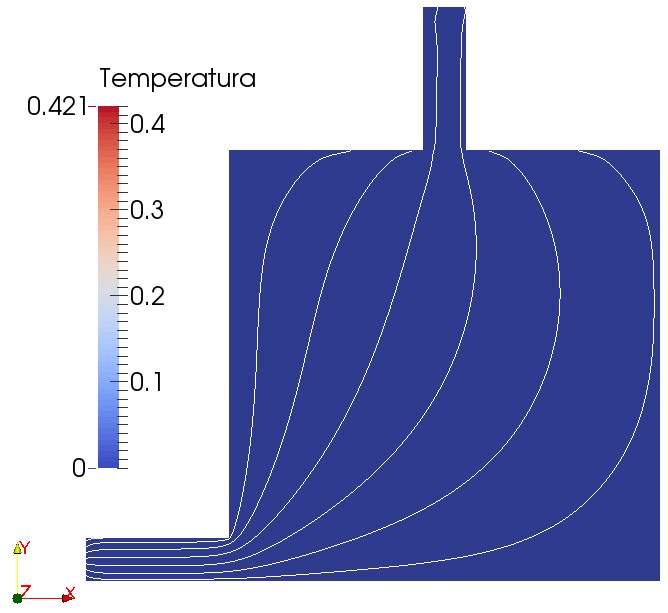
\includegraphics[width=0.5\textwidth]{ri-portada.png}
}%
{figs/ri05.ogv} % video filename
\end{center}

\end{frame}


\begin{frame}
{Ejemplos de aplicación}
{Fluidodinámica en una fuente fría de neutrones}
Distintos comportamientos según el $Ri$ obtenido:
\begin{itemize}
\item $Ri=84$:
\end {itemize}

\begin{center}
\movie[width=0.7\textwidth,showcontrols=true]
{% placeholder = text or image
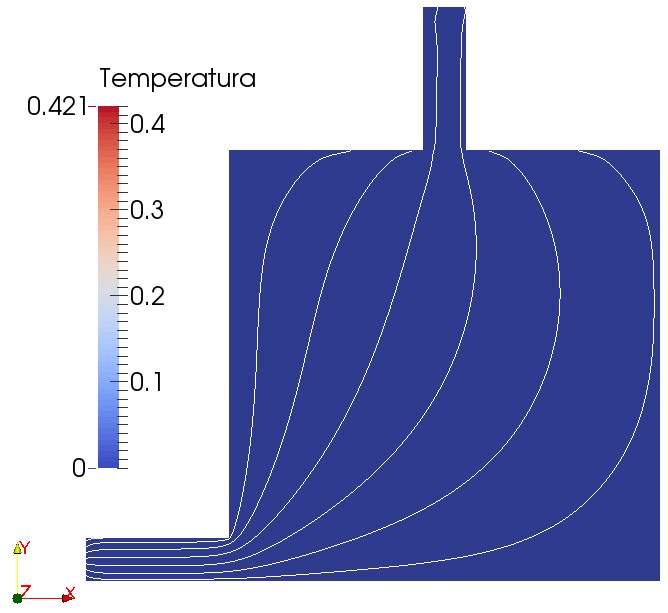
\includegraphics[width=0.5\textwidth]{ri-portada.png}
}%
{figs/ri84.ogv} % video filename
\end{center}

\end{frame}




\begin{frame}
{Ejemplos de aplicación}
{Fluidodinámica en una fuente fría de neutrones}

A mayor altura $H$ del intercambiador de calor, mayor caudal obtenido:

\begin{table}[h!]
  \centering
  \begin{tabular}{ c c c c c c c } 
      \hline
      \multicolumn{1}{c}{$f_0$ $[W/m^3]$} & \multicolumn{1}{c}{$H / \Delta z$} & \multicolumn{1}{c}{$Ri$} & \multicolumn{1}{c}{$\Delta T$ $[K]$} & \multicolumn{1}{c}{$Q$$[m^3/s]$}& \multicolumn{1}{c}{$\Delta p$ $[Pa]$} \\ \hline
      \multirow{3}{*}{$2\cdot10^4$} & $1$ & 3.4 & 0.7 & $3.2 \cdot 10^{-3}$ & 613 \\
                         & $5$ & 1 & 0.5 & $4.2 \cdot 10^{-3}$ & 614 \\
                         & $10$ & 0.5 & 0.3 & $4.5 \cdot 10^{-3}$ & 617 \\ \hline
      \multirow{3}{*}{$2\cdot10^5$} & $1$ & 6.5 & 3.6 & $4.4 \cdot 10^{-3}$ & 595 \\
                         & $5$ & 1.7 & 2.8 & $7.6 \cdot 10^{-3}$ & 605 \\
                         & $10$ & 0.9 & 2.2 & $9.0 \cdot 10^{-3}$ & 620 \\ \hline
      \multirow{3}{*}{$2\cdot10^6$} & $1$ & 10.6 & 24 & $8.9 \cdot 10^{-3}$ & 465 \\
                         & $5$ & 2.2 & 18 & $1.7 \cdot 10^{-2}$ & 580 \\
                         & $10$ & 0.9 & 11.6 & $2.1 \cdot 10^{-2}$ & 700 \\ \hline
   \end{tabular}   
   \caption[Principales resultados del cálculo para el análisis de la fuente fría variando la magnitud de la fuente interna y la altura del sistema de enfriamiento]
   {Principales resultados del cálculo para el análisis de la fuente fría variando la magnitud de la fuente interna y la altura del sistema de enfriamiento.}
   \label{tab-deuterio}
\end{table}

\end{frame}


\begin{frame}
{Ejemplos de aplicación}
{Fluidodinámica en una fuente fría de neutrones}

Análisis de métodos de resolución del sistema de ecuaciones de residuos:

\begin{figure}
\centering{}
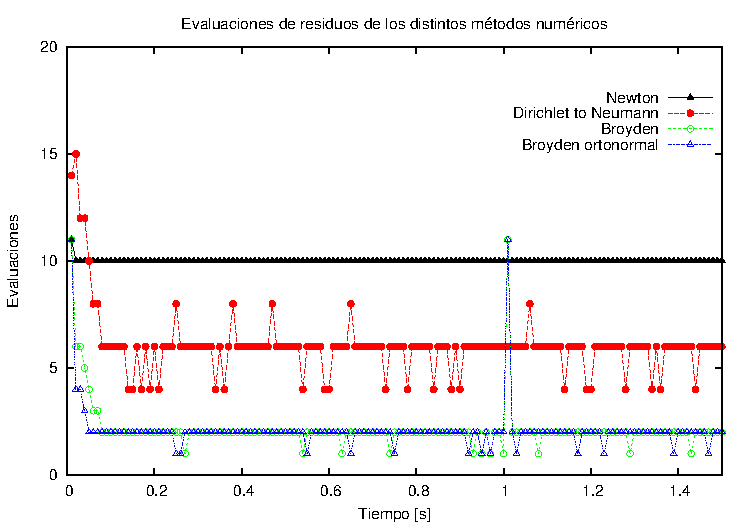
\includegraphics[scale=0.7]{evaluaciones-ff.pdf}
\end{figure}

\end{frame}












\subsection{Análisis del segundo sistema de parada de un reactor de investigación}

\begin{frame}
{Ejemplos de aplicación}
{Análisis del segundo sistema de parada de un reactor de investigación}

Esquema del Segundo Sistema de Parada (SSP) del RA-10:

\begin{figure}
\centering{}
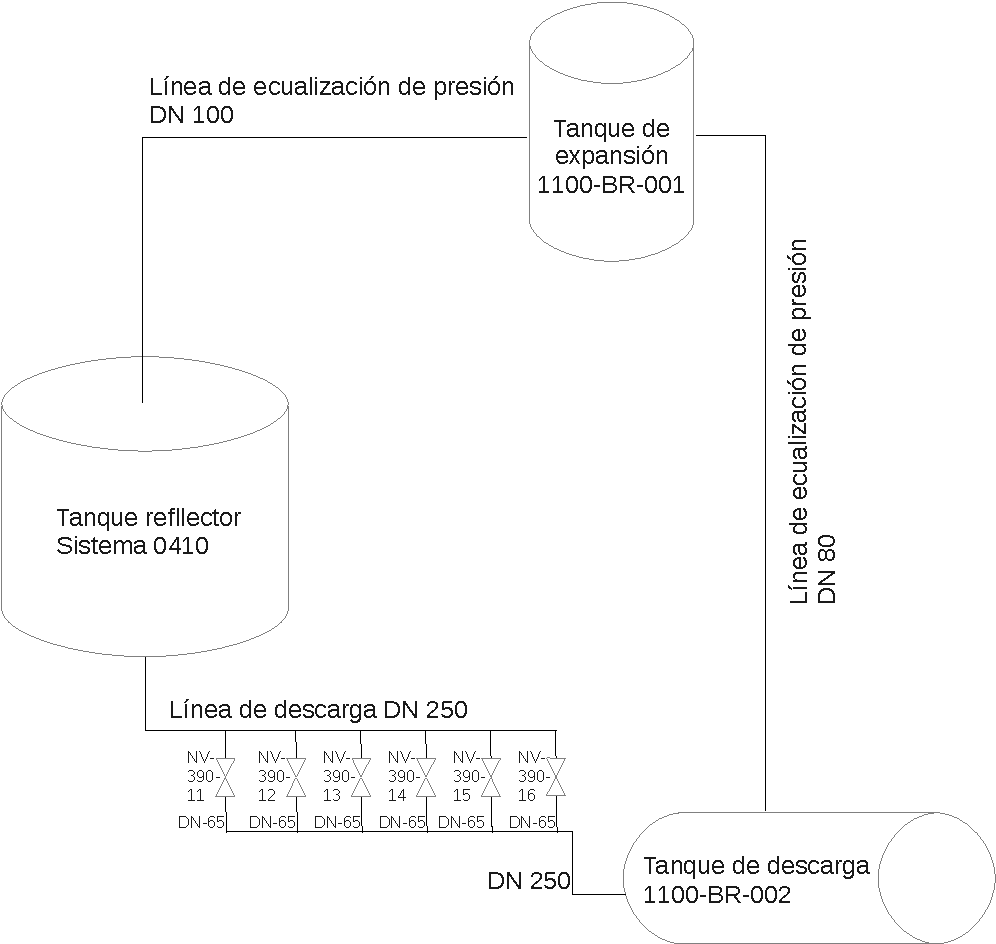
\includegraphics[scale=0.42]{SSP.pdf}
\end{figure}

\end{frame}

\begin{frame}
{Ejemplos de aplicación}
{Análisis del segundo sistema de parada de un reactor de investigación}

Subdominios de análisis:

\begin{itemize}
\item <2-> Subsistema del tanque del reflector,
\item <3-> Subsistema de la red hidráulica de descarga,
\item <4-> Subsistema de la red hidráulica de ecualización de presiones.
\end{itemize}

\end{frame}

\begin{frame}
{Ejemplos de aplicación}
{Análisis del segundo sistema de parada de un reactor de investigación}

Subdominios de análisis:

\begin{itemize}
\item Subsistema del tanque del reflector (0-D),
\item Subsistema de la red hidráulica de descarga (3-D),
\item \sout{Subsistema de la red hidráulica de ecualización de presiones}.
\end{itemize}

\end{frame}

% \tiny
% \scriptsize
% \footnotesize
% \small	
% \normalsize
% \large
% \Large
% \LARGE
% \huge
% \Huge

\footnotesize
\begin{frame}
{Ejemplos de aplicación}
{Análisis del segundo sistema de parada de un reactor de investigación}

Subsistema 0-D:

\begin{equation*}
\ddot{h} h + \frac{\dot{h}^2}{2}\left( 1- \left(\frac{A_T}{A_D} \right)^2 \right) + g \Delta h_{red} + \ddot{h}  l_D = 
\frac{p_{atm}-p_1^1}{\rho} + \Delta \hat{u}
\label{eq-tanque}
\end{equation*}
donde $p_1^1$ es la presión en la interfaz de acople,
$A_T$ es la área transversal del tanque del reflector, 
$A_D$ es la sección transversal de la línea de descarga,
$\Delta h_{red}$ es la altura total de la columna de líquido en el subsistema,
$l_D$ es la longitud total de cañerías en el subsistema,
$p_{atm}$ es la presión sobre la superficie libre,
y $\rho$ es la densidad del agua.
$\Delta \hat{u}$ representa la pérdida de carga por unidad de masa y puede modelarse como:

\begin{equation*}
\Delta \hat{u} = \frac {1} {2} {v_D}^2 \left( \frac {f_D l_D}{D} + \sum_i K_i \right)
\end{equation*}
donde $v_D$ es la velocidad del fluido en la línea de descarga,
(que puede escribirse en términos de $\dot{h}$),
$\frac {f_D*l_D}{D}$ es el factor de pérdida de carga distribuida en las tuberías,
(en función del factor de Darcy $f_D$, la longitud de tuberías $l_D$ y el diámetro de las mismas $D$)
y $\sum_i K_i$ es la sumatoria de factores de pérdida de carga concentrada.

\end{frame}

\normalsize
\begin{frame}
{Ejemplos de aplicación}
{Análisis del segundo sistema de parada de un reactor de investigación}

\begin{table}[]
\centering
\begin{tabular}{|l|l|}
\hline
Parámetro        & Valor          \\ \hline
$A_T$            & 5.30 $m^2$     \\ \hline
$A_D$            & 0.05 $m^2$     \\ \hline
$\Delta h_{red}$ & $h$ + 4.98 $m$ \\ \hline
$l_D$            & 11.98 $m$      \\ \hline
$p_{atm}$        & 92000 $Pa$     \\ \hline
$\rho$           & 998 $Kg/m^3$   \\ \hline
$D$              & 0.254 $m$      \\ \hline
$\sum_i K_i$     & 1.13           \\ \hline
\end{tabular}
\caption{Parámetros del subsistema del tanque del reflector con acople de porción de red hidráulica}
\label{tabla-tanque}
\end{table}

\end{frame}


\footnotesize
\begin{frame}
{Ejemplos de aplicación}
{Análisis del segundo sistema de parada de un reactor de investigación}

Subsistema 3-D:

\begin{equation*}
\left\{ \begin{array}{l}
\displaystyle \frac{\partial \bar{U} }{\partial t} + ( \bar{U} \cdot \nabla) \bar{U} = - \frac {\nabla P^*}{\rho} + 
\nabla \cdot \left[ \left( \nu + \nu_T \right) \left( \nabla \bar{U} + \nabla U^T \right) \right] +\bar{f} \\
\nabla \cdot \bar{U} =0 \\
\displaystyle \nu_T = c_\mu \frac{\kappa^2}{\epsilon} \\
\displaystyle \frac{\partial \kappa}{\partial t} + ( \bar{U} \cdot \nabla) \kappa = \frac{c_\mu} {2}{\kappa^2}{\epsilon} \left | \nabla \bar{U} + \nabla\bar{U}^T \right | ^2  
+ \nabla \cdot \left( c_\mu \frac{\kappa^2}{\epsilon} \nabla \kappa \right) - \epsilon \\
\displaystyle \frac{\partial {\epsilon}}{\partial t} + ( \bar{U} \cdot \nabla) \epsilon = \frac{c_1} {2} \kappa \left | \nabla \bar{U} + \nabla \bar{U}^T \right | ^2
+ \nabla \cdot \left( c_{\epsilon} \frac{\kappa^2}{\epsilon} \nabla \epsilon \right) - c_2 \frac{\epsilon}{\kappa}
\label{eq-mani}
\end{array} \right.
\end{equation*}
donde $\bar{f}$ es una fuerza volumétrica, 
$\kappa$ es la energía cinética turbulenta, $\epsilon$ es la disipación viscosa de energía turbulenta,
$\nu_T$ es la viscosidad turbulenta y $P^*$ es la presión efectiva del sistema, que se calcula como
$\displaystyle P^* = P + \frac {2}{3}\kappa$.
Las variables mayúsculas refieren a valores medios estadísticos.
Los parámetros de las ecuaciones de transporte de $\kappa$ y $\epsilon$ toman los siguientes valores:
$c_\mu=0.09$, $c_1=0.126$, $c_2=1.92$ y $c_\epsilon=0.07$ \cite{durbin}.

\end{frame}

\normalsize
\begin{frame}
{Ejemplos de aplicación}
{Análisis del segundo sistema de parada de un reactor de investigación}

Estrategia de resolución: 
\begin{itemize}
\item Elección de variables: $\{p,Q\}$
\item <2->Ecuaciones de continuidad:
\begin{equation*}
\left\{ \begin{array}{l}
p_1^1 = p_2^1 \\
Q_1^1 = Q_2^1
\end{array}
\right.
\end{equation*}
\item <3-> Selección de condiciones de borde:
    \begin{itemize}
    \item Subsistema 0-D: condición de tipo $Neumann$
    \item Subsistema 3-D: condición de tipo $Dirichlet$
    \end{itemize}
\item <4-> Ecuaciones de residuos:

\begin{equation*}
\left\{ \begin{array}{l}
(R_{p,Q})_{1}^{1} =Q_1^{1,guess} - Q_1^{1,calc}(p_1^{1,guess}) \\
(R_{p,Q})_{2}^{1} =p_2^{1,guess} - p_2^{1,calc}(Q_2^{1,guess})
\end{array}
\right.
\end{equation*}

\end{itemize}

\end{frame}



\begin{frame}
{Ejemplos de aplicación}
{Análisis del segundo sistema de parada de un reactor de investigación}
Análisis de la descarga del SSP:
\begin{figure}
\centering{}
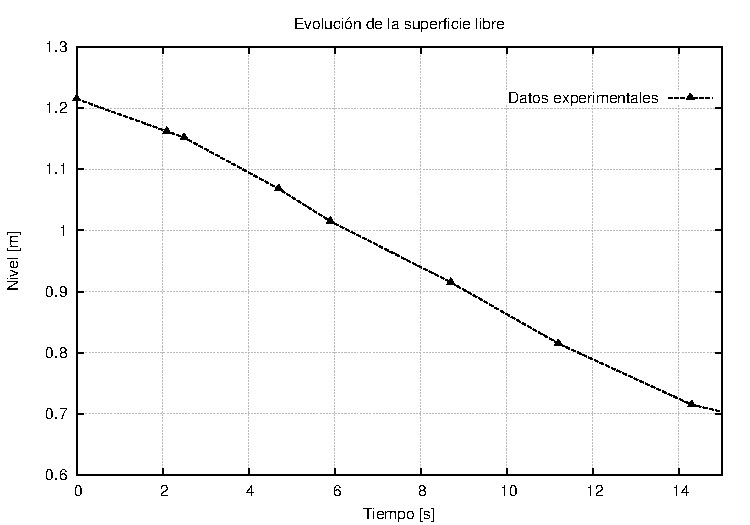
\includegraphics[scale=0.7]{hvst1.pdf}
\end{figure}
\end{frame}
\begin{frame}
{Ejemplos de aplicación}
{Análisis del segundo sistema de parada de un reactor de investigación}
Análisis de la descarga del SSP:
\begin{figure}
\centering{}
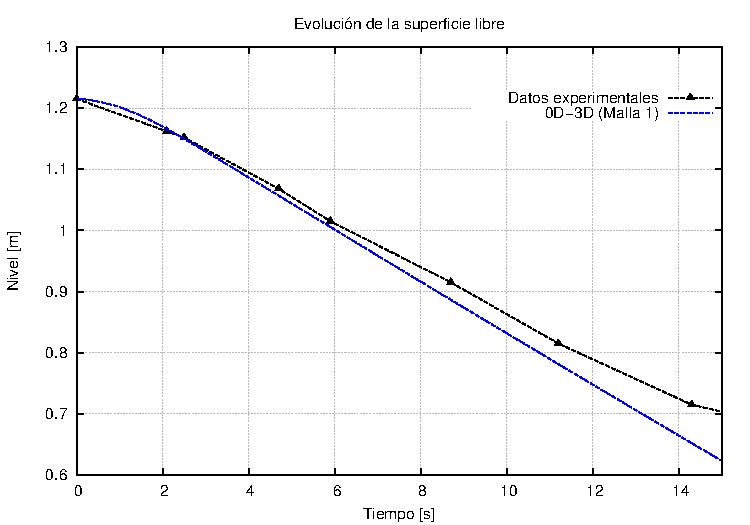
\includegraphics[scale=0.7]{hvst2.pdf}
\end{figure}
\end{frame}
\begin{frame}
{Ejemplos de aplicación}
{Análisis del segundo sistema de parada de un reactor de investigación}
Análisis de la descarga del SSP:
\begin{figure}
\centering{}
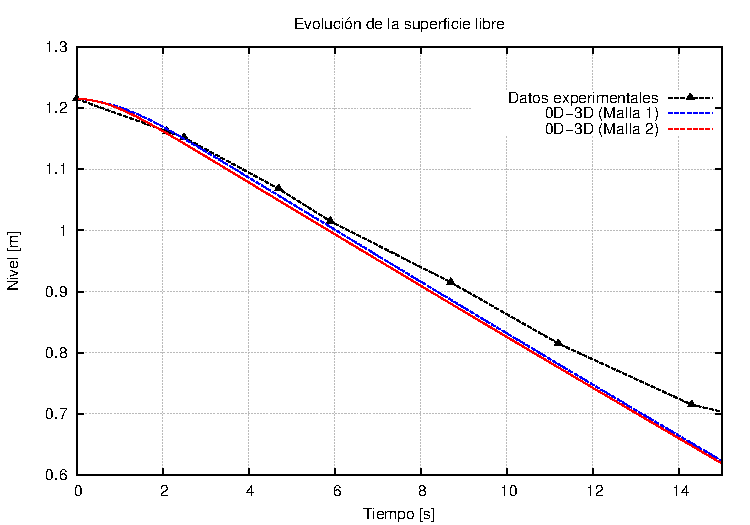
\includegraphics[scale=0.7]{hvst3.pdf}
\end{figure}
\end{frame}
\begin{frame}
{Ejemplos de aplicación}
{Análisis del segundo sistema de parada de un reactor de investigación}
Análisis de la descarga del SSP:
\begin{figure}
\centering{}
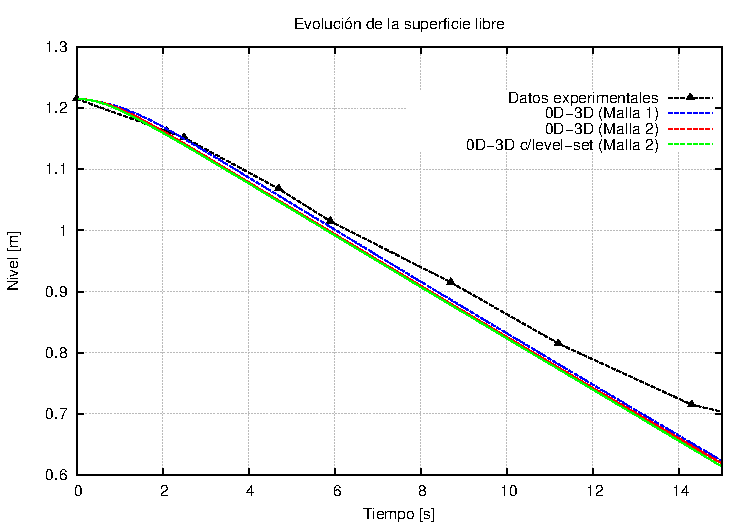
\includegraphics[scale=0.7]{hvst4.pdf}
\end{figure}
\end{frame}
\begin{frame}
{Ejemplos de aplicación}
{Análisis del segundo sistema de parada de un reactor de investigación}
Análisis de la descarga del SSP:
\begin{figure}
\centering{}
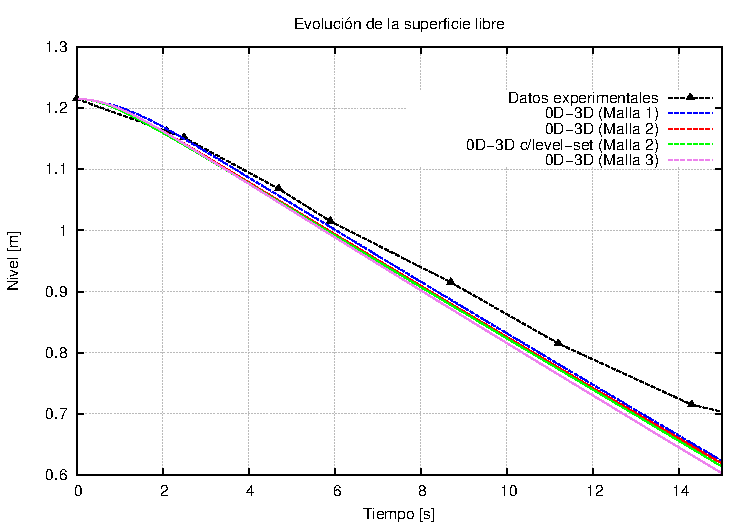
\includegraphics[scale=0.7]{hvst5.pdf}
\end{figure}
\end{frame}
\begin{frame}
{Ejemplos de aplicación}
{Análisis del segundo sistema de parada de un reactor de investigación}
Análisis de la descarga del SSP:
\begin{figure}
\centering{}
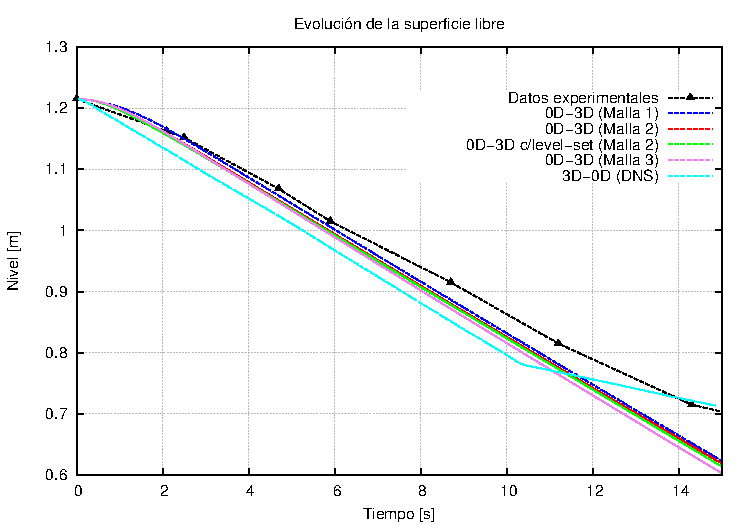
\includegraphics[scale=0.7]{hvst6.pdf}
\end{figure}
\end{frame}
\begin{frame}
{Ejemplos de aplicación}
{Análisis del segundo sistema de parada de un reactor de investigación}
Análisis de la descarga del SSP:
\begin{figure}
\centering{}
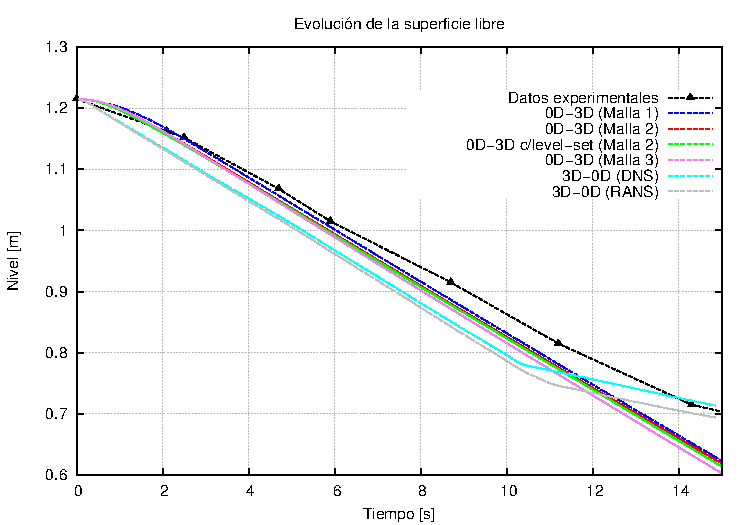
\includegraphics[scale=0.7]{hvst7.pdf}
\end{figure}
\end{frame}

\begin{frame}
{Ejemplos de aplicación}
{Análisis del segundo sistema de parada de un reactor de investigación}
Análisis de sensibilidad de resultados ante válvula en falla
\begin{figure}
\centering{}
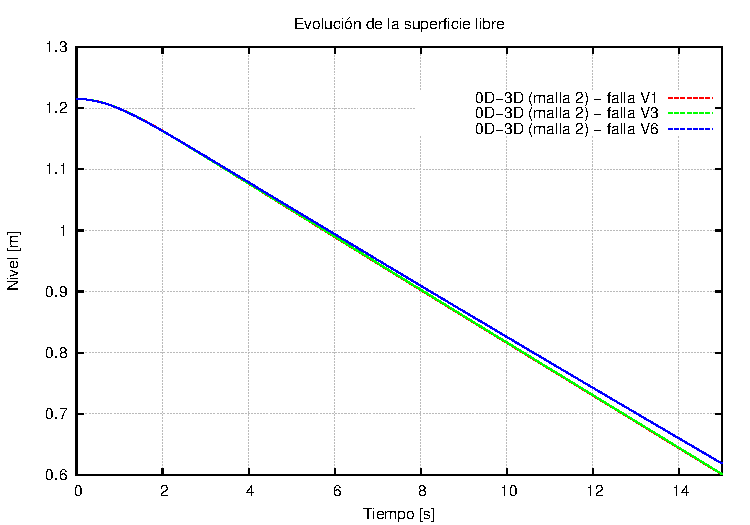
\includegraphics[scale=0.7]{hvstv.pdf}
\end{figure}
\end{frame}

\begin{frame}
{Ejemplos de aplicación}
{Análisis del segundo sistema de parada de un reactor de investigación}
Transporte de superficie libre en cañerías
\begin{equation*}
%\left\{ \begin{array}{rcl}
%\displaystyle \frac{\partial\phi}{\partial t}+ (\bar{u} \cdot \nabla) \phi &=& 0
\frac{\partial\phi}{\partial t}+ (\bar{u} \cdot \nabla) \phi = 0
\label{eq-ls}
%\end{array} \right.
\end{equation*}
\end{frame}
\begin{frame}
{Ejemplos de aplicación}
{Análisis del segundo sistema de parada de un reactor de investigación}
Transporte de superficie libre en cañerías
\begin{center}
\movie[width=1\textwidth,showcontrols=true]
{% placeholder = text or image
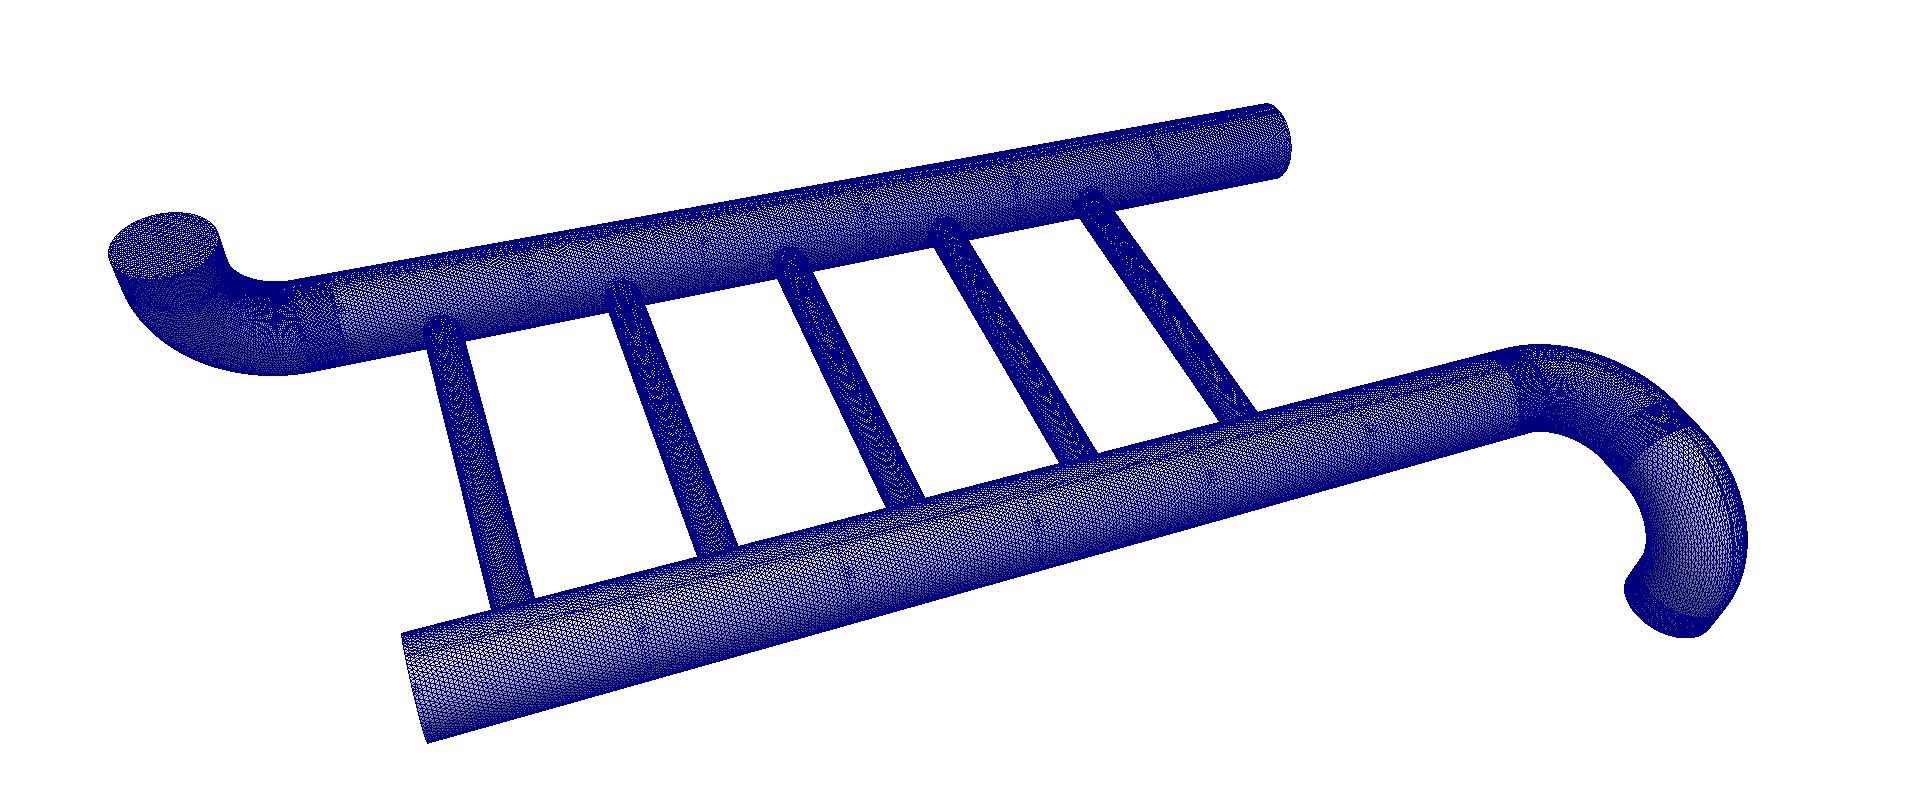
\includegraphics[width=1\textwidth]{ls-portada.png}
}%
{figs/ls.ogv} % video filename
\end{center}
\end{frame}
\begin{frame}
{Ejemplos de aplicación}
{Análisis del segundo sistema de parada de un reactor de investigación}
Transporte de superficie libre en cañerías
\begin{figure}
\centering{}
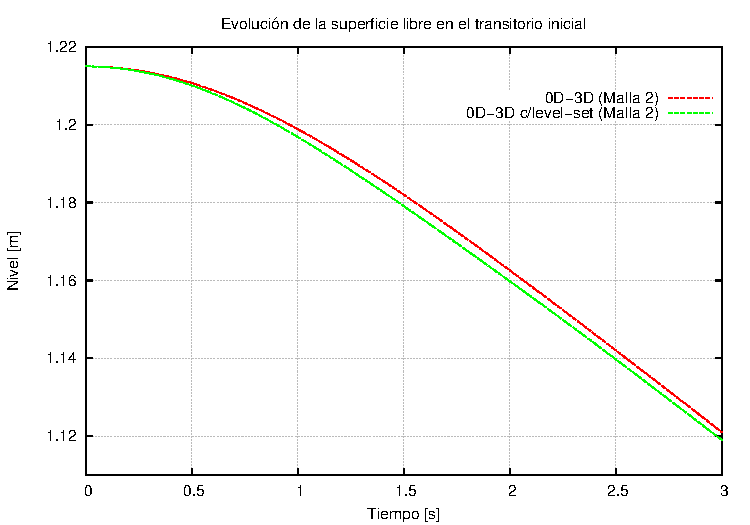
\includegraphics[scale=0.7]{hvstlsZoom.pdf}
\end{figure}
\end{frame}





\begin{frame}
{Ejemplos de aplicación}
{Análisis del segundo sistema de parada de un reactor de investigación}
Estudio de métodos numéricos para la resolución del sistema de residuos
\begin{figure}
\centering{}
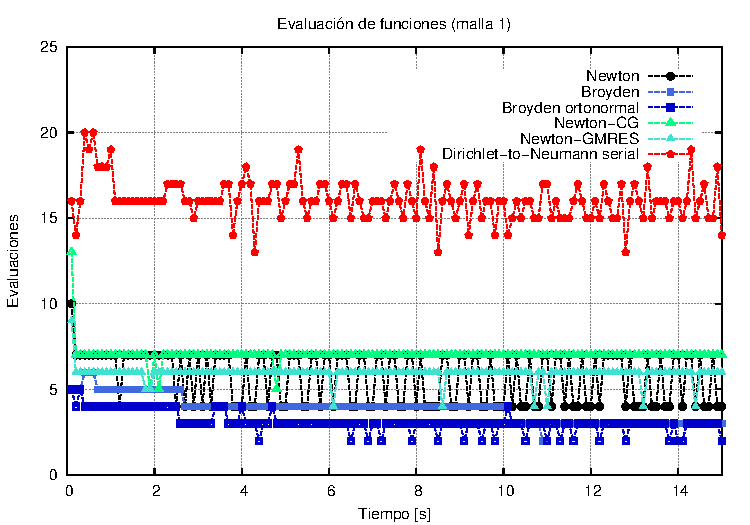
\includegraphics[scale=0.7]{nonlinear_fevals_ssp.pdf}
\end{figure}
\end{frame}







\subsection{Resolución de redes hidráulicas de múltiples componentes}

\begin{frame}
{Ejemplos de aplicación}
{Resolución de redes hidráulicas de múltiples componentes}
Descomposición disjunta de dominios en un modelo de red hidráulica con 8 incógnitas reducidas en las interfaces de acoplamiento:

\begin{figure}[ht]
\centering{}
\begin{tikzpicture}
[scale=0.8, every node/.style={scale=0.8}]

% Nodos
\node [label={\small $S_3$}] at (0em,0em) (n8) {};

\node [right of=n8, xshift=3em, yshift=-2em, align=center] (n13) {\small $v_{3}^{3}, \quad v_{5}^{1},$ \\ $P_{3}^{3}$ \quad $P_{5}^{1}$};
\node [right of=n13, xshift=3em, yshift=-2em, label={\small $S_5$}] (n14) {};
\node [right of=n14, xshift=2em, yshift=-2em] (n16) {\small $CB_{5}^{3}$};
\node [right of=n14, xshift=2em, yshift=2em] (n15) {\small $CB_{5}^{2}$};

\node [right of=n8, xshift=3em, yshift=2em, align=center] (n9) {\small $v_{3}^{2}, \quad v_{4}^{1},$ \\ $P_{3}^{2}$ \quad $P_{4}^{1}$};
\node [right of=n9, xshift=3em, yshift=0em, label={\small $S_4$}] (n10) {};
\node [right of=n10, xshift=2em, yshift=-2em] (n12) {\small $CB_{4}^{3}$};
\node [right of=n10, xshift=2em, yshift=2em] (n11) {\small $CB_{4}^{2}$};

\node [left of=n8, xshift=-3em, yshift=2em, align=center] (n7) {\small $v_{1}^{3}, \quad v_{3}^{1},$ \\ $P_{1}^{3}$ \quad $P_{3}^{1}$};
\node [left of=n7, xshift=-4em, yshift=3em, label={\small $S_1$}] (n2) {};
\node [left of=n2, xshift=-1em, yshift=-0em] (n1) {\small $CB_{1}^{1}$};

\node [right of=n2, xshift=4em, yshift=3em, align=center] (n3) {\small $v_{1}^{2}, \quad v_{2}^{1},$ \\ $P_{1}^{2}$ \quad $P_{2}^{1}$};
\node [right of=n3, xshift=3em, yshift=0em, label={\small $S_2$}] (n4) {};
\node [right of=n4, xshift=2em, yshift=2em] (n5) {\small $CB_{2}^{2}$};
\node [right of=n4, xshift=2em, yshift=-2em] (n6) {\small $CB_{2}^{3}$};

% Conexiones
\draw[|-] (n1.east) to [in=180, out=0] (n2.center);
\draw[-o] (n2.center) to[in=180, out=0] (n3.west);
\draw[-o] (n2.center) to[in=180, out=0] (n7.west);

\draw[o-] (n3.east) to[in=180, out=0] (n4.center);
\draw[-|] (n4.center) to[in=180, out=0] (n5.west);
\draw[-|] (n4.center) to[in=180, out=0] (n6.west);

\draw[o-] (n7.east) to[in=180, out=0] (n8.center);
\draw[-o] (n8.center) to[in=180, out=0] (n9.west);
\draw[-o] (n8.center) to[in=180, out=0] (n13.west);

\draw[o-] (n9.east) to[in=180, out=0] (n10.center);
\draw[-|] (n10.center) to[in=180, out=0] (n11.west);
\draw[-|] (n10.center) to[in=180, out=0] (n12.west);

\draw[o-] (n13.east) to[in=180, out=0] (n14.center);
\draw[-|] (n14.center) to[in=180, out=0] (n15.west);
\draw[-|] (n14.center) to[in=180, out=0] (n16.west);

\end{tikzpicture}
%~ \caption[Descomposición disjunta de dominios en el modelado de redes hidráulicas]
%~ {Descomposición disjunta de dominios en un modelo de red hidráulica con 16 incógnitas en las interfaces de acoplamiento.
%~ La incógnita $v_{i}^{j}$ refiere a la velocidad media en el extremo $j$ del subsistema $i$.
%~ La incógnita $P_{i}^{j}$ agrupa las presiones estática y dinámica medias en el extremo $j$ del subsistema $i$.
%~ Las incógnitas pueden reducirse rápidamente a la mitad aplicando relaciones de continuidad de campos de variables.}
%~ \label{net16}
\end{figure}

\end{frame}


\begin{frame}
{Ejemplos de aplicación}
{Resolución de redes hidráulicas de múltiples componentes}

\begin{itemize}
\item Cada subsistema se modela con ecuaciones de continuidad y de conservación de energía.
\item <2-> Ecuaciones de residuos:
\begin{equation*}
\left \{
\begin{array}{rl}
R_1 =& v_1^{2,guess} - v_1^{2,calc}(CB_1^1, P_1^{2,guess}, P_1^{3,guess}) \\
R_2 =& v_1^{3,guess} - v_1^{3,calc}(CB_1^1, P_1^{2,guess}, P_1^{3,guess}) \\
R_3 =& P_2^{1,guess} - P_2^{1,calc}(v_2^{1,guess}, CB_2^2, CB_2^3) \\
...
\end{array}
\right .
\end{equation*}
\end{itemize}
\end{frame}

\begin{frame}
{Ejemplos de aplicación}
{Resolución de redes hidráulicas de múltiples componentes}
%~ 
Redes hidráulicas con regímenes de flujo laminar:

\begin{figure}[ht]
	\begin{minipage}{0.48\linewidth}
      \centering
      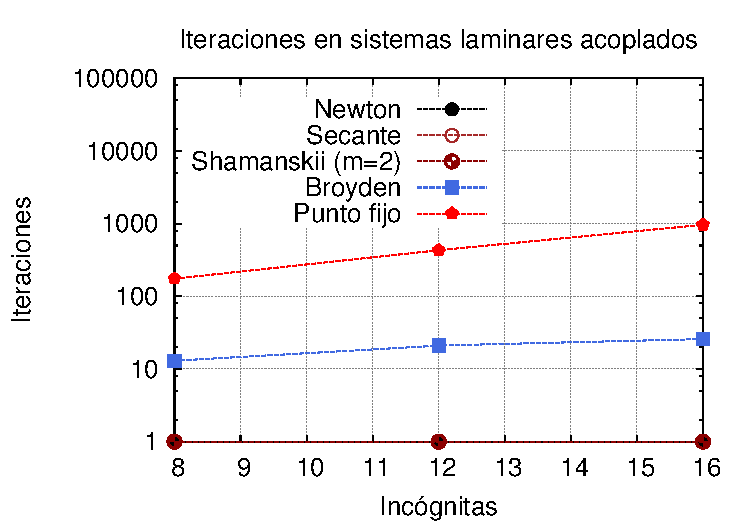
\includegraphics[scale=0.42]{net_linear_its.pdf}
		%~ \caption[]{t=0 s}
		%~ \label{asd}	
	\end{minipage}
	\begin{minipage}{0.48\linewidth}
		\centering
		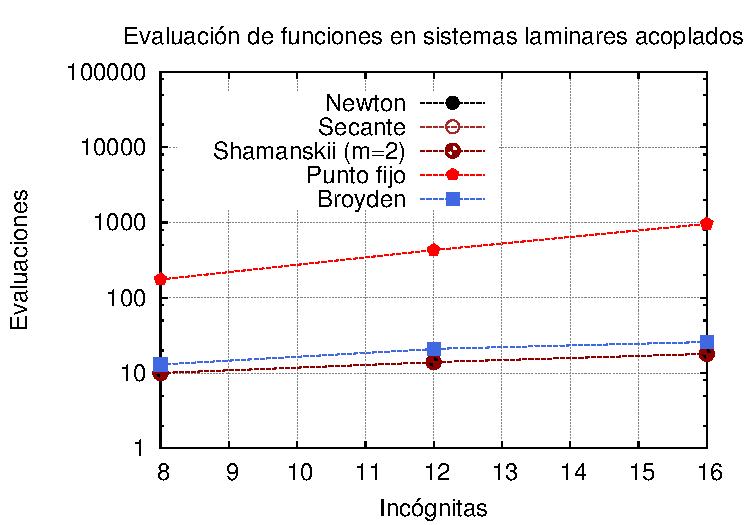
\includegraphics[scale=0.42]{net_linear_fevals.pdf}
		%~ \caption[]{t=40 s}
		%~ \label{asd}	
	\end{minipage}
\end{figure}
\end{frame}
\begin{frame}
{Ejemplos de aplicación}
{Resolución de redes hidráulicas de múltiples componentes}
Redes hidráulicas con regímenes de flujo laminar:
\begin{figure}
\centering
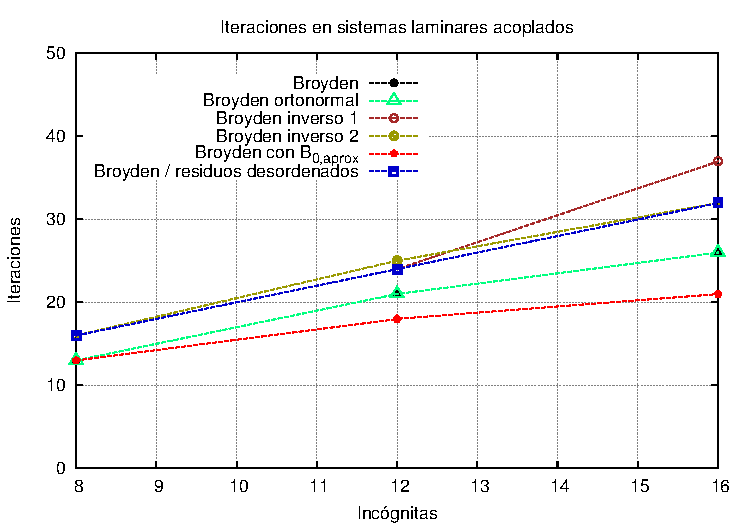
\includegraphics[scale=0.6]{net_linear_its_broy.pdf}
\end{figure}
\end{frame}

\begin{frame}
{Ejemplos de aplicación}
{Resolución de redes hidráulicas de múltiples componentes}

Redes hidráulicas con regímenes de flujo turbulento:

\begin{figure}[ht]
\centering
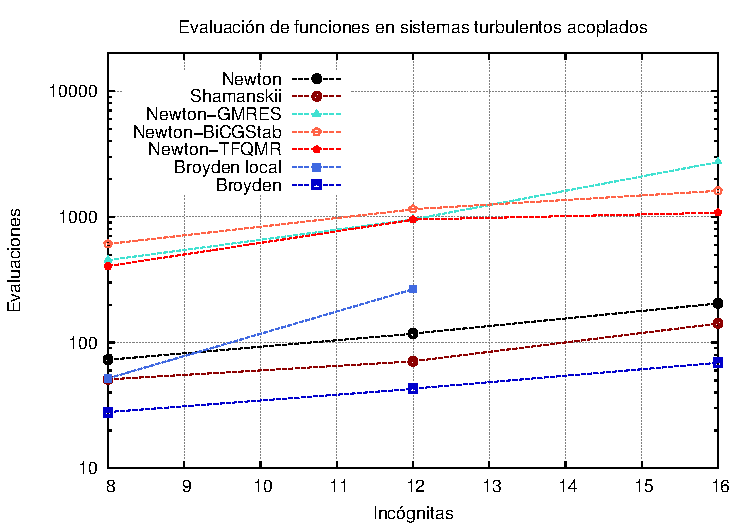
\includegraphics[scale=0.6]{net_nonLinear_fevals.pdf}
\end{figure}
\end{frame}





\subsection{Extensión a problemas acoplados en modelos de núcleo}

\begin{frame}
{Ejemplos de aplicación}
{Extensión a problemas acoplados en modelos de núcleo}

La estrategia de resolución mediante acoplamiento de códigos desarrollada puede extenderse para resolver sistemas genéricos de ecuaciones acopladas:
\begin{itemize}
  \item <2-> Las variables de acople no necesariamente deben corresponder a condiciones de borde
  \item <3-> Las variables de acople no necesariamente deben agruparse en pares
\end{itemize}
\visible<4->{
Objetivo: Modelar la dinámica del núcleo de un reactor nuclear mediante acoplamiento de códigos que resuelvan diferentes fenómenos físicos:
}
\begin{itemize}
  \item <5-> Neutrónica
    \begin{itemize}
    \item Distribución de flujo neutrónico
    \item Quemado de elementos combustibles
    \item Movimiento de barras
    \end{itemize}
  \item <6-> Termohidráulica
    \begin{itemize}
    \item Distribución de temperaturas
    \item Distribución de densidad de refrigerante
    \end{itemize}
  \item <7-> $Swelling$ de pastillas % Altera propiedades termicas (k)
  \item <8-> $Pellet-cladding$ interaction % Altera propiedades mecanicas (eps) termicas (k)
  \item <9-> Otros
\end{itemize}

\end{frame}


\begin{frame}
{Ejemplos de aplicación}
{Extensión a problemas acoplados en modelos de núcleo}
Primer modelo simplificado:
acoplamiento neutrónico-termohidráulico en cálculo de quemado de elementos combustibles.
Asumimos que:
  \begin{itemize}
    \item <2-> No hay movimiento de barras
    \item <3-> No se modela comportamiento de materiales
    \item <4-> Las secciones eficaces neutrónicas están condensadas por zonas y grupos de energía en previos cálculos de celda, y tienen dependencia con el quemado y con variables termohidráulicas
   \end{itemize}

\end{frame}


\scriptsize
\begin{frame}
{Ejemplos de aplicación}
{Extensión a problemas acoplados en modelos de núcleo}
Modelo neutrónico:

Cálculo de flujo neutrónico:
\begin{equation*}
\Delta \bar{\phi} = \frac{1}{k_{eff}}\Sigma \bar{\phi}
\label{eq-nucleo}
\end{equation*}
donde $\bar{\phi}$ es una función vectorial con el valor del flujo neutrónico en cada punto del espacio para diferentes grupos de energía,
$\Sigma$ es la matriz de secciones eficaces asociada a diferentes reacciones para diferentes grupos de energía,
y $k_{eff}$ es el factor de multiplicación del reactor.

\visible<2->{Cálculo de secciones eficaces:
\begin{equation*}
\Sigma = \Sigma \left ( N_{ref}, T_{ref}, T_{comb} \right )
\label{eq-sigma}
\end{equation*}

donde $N_{ref}$ es la densidad del refrigerante, $T_{ref}$ es la temperatura del refrigerante, $T_{comb}$ es la temperatura del combustible , 
y $B$ es el valor histórico de quemado  del material \cite{lamarsh}.
}

\visible<3->{
Cálculo de distribución de potencia:
\begin{equation*}
P = \int_{vol} E_{fis,i} \Sigma_{fis,i} \phi_{i}
\label{power}
\end{equation*}
donde $E_{fis,i}$ es la energía liberada por fisiones ocurridas en el rango de energía $i$,
$\Sigma_{fis,i}$ es la sección eficaz de fisión condensada en el grupo de energía $i$ y
$\phi_{i}$ es la componente del flujo neutrónico también condensada en el grupo de energía $i$.
}

\end{frame}



\normalsize
\begin{frame}
{Ejemplos de aplicación}
{Extensión a problemas acoplados en modelos de núcleo}

El núcleo se modela como un único canal, en contacto con una única estructura que genera energía, con diámetro del $pin$ y altura equivalente a la altura de la suma total de $pines$.

\visible<2->{La transferencia de calor a través de las estructuras de combustibles se estudia con un modelo de difusión.
}

\visible<3->{El modelo termohidráulico del refrigerante considera ecuaciones de mezcla del fluido en fases líquida y gaseosa:
\begin{itemize}
\item 2 Ecuaciones de continuidad;
\item 2 Ecuaciones de momento unidimensionales;
\item 2 Ecuaciones de conservación de energía.
\end{itemize}
}
\end{frame}

\normalsize
\begin{frame}
{Ejemplos de aplicación}
{Extensión a problemas acoplados en modelos de núcleo}

Estrategia de resolución:

\begin{itemize}
\item <2-> El código neutrónico recibe como $guess$ distribución de secciones eficaces y calcula distribución de potencia.
\item <3-> El código termohidráulico recibe como $guess$ distribución de potencias y calcula distribución de temperaturas y densidades.
\item <4-> Las variables se acoplan en zonas físicas predefinidas.
\item <5-> La evolución se discretiza en intervalos de 5 o 10 días.
\item <6-> El valor del quemado inicial es $B(\bar{x})=0$ en todo el dominio.
\item <7-> En cada intervalo temporal se actualiza el valor de $B$ por zonas físicas, considerando la distribución de potencias constante.

\end{itemize}

\end{frame}



\scriptsize
\begin{frame}
{Ejemplos de aplicación}
{Extensión a problemas acoplados en modelos de núcleo}

Acoplamiento de \textbf{Fermi} y \textbf{RELAP5} en modelo simple de núcleo:

\begin{figure}[ht]
	\begin{minipage}{0.6\linewidth}
      \centering
      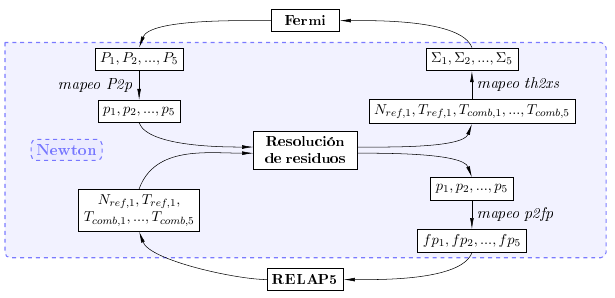
\includegraphics[scale=0.43]{esq-fermi-relap.png}
		%~ \caption[]{t=0 s}
		%~ \label{asd}	
	\end{minipage}
	\begin{minipage}{0.35\linewidth}
		\centering
		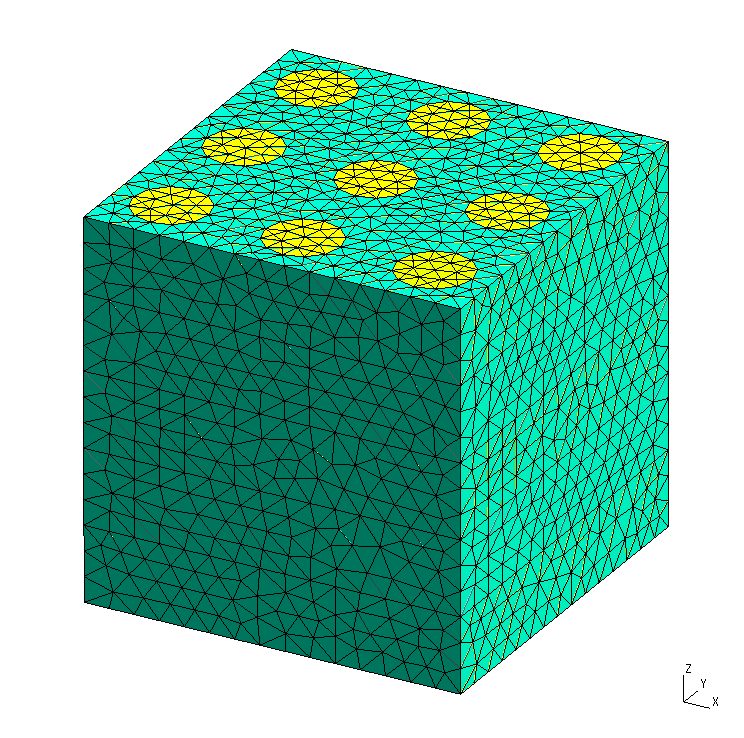
\includegraphics[scale=0.16]{fuel_z5.png}
		%~ \caption[]{t=40 s}
		%~ \label{asd}	
	\end{minipage}
\end{figure}
\visible<2->{
\begin{table}[h]
  \centering
  \begin{tabular}{c c c c cc } \hline
      \multicolumn{1}{c}{Método} & \multirow{1}{*}{$\Delta$t} & \multicolumn{1}{c}{Extrapolación} & \multicolumn{1}{c}{Extrapolación}  & \multicolumn{1}{c}{Evaluaciones} & \multicolumn{1}{c}{Tiempo} \\ % \hline
      \multicolumn{1}{c}{no lineal} & [días] & \multicolumn{1}{c}{de $\bar{x}^n$} & \multicolumn{1}{c}{de $\mathbb{J}^n$} & \multicolumn{1}{c}{totales} & \multicolumn{1}{c}{total [s]}\\ \hline %\hline
      Broyden & 10 & $\mathscr{O}(1)$ & $\mathscr{O}(1)$ & 85 & 610 \\ %\hline
      Picard & 10 & $\mathscr{O}(1)$ & - & 68 & 684 \\ %\hline
      % Punto fijo & 10 & $\mathscr{O}(1)$ & - & 87 & 628  \\ %\hline
      Shamanskii & 10 & $\mathscr{O}(1)$ & $\mathscr{O}(0)$& 370 & 2663  \\ \hline
   \end{tabular}   
   \caption[Evaluaciones totales y tiempo total requerido por cada método no lineal en cálculo de quemado con \textbf{RELAP5} y \textbf{Fermi}]
   {\scriptsize Evaluaciones totales y tiempo total requerido por cada método no lineal.}
   \label{tabla-relap-fermi}
\end{table}
}

\end{frame}




\normalsize
\begin{frame}
{Ejemplos de aplicación}
{Extensión a problemas acoplados en modelos de núcleo}

Acoplamiento de \textbf{PUMA} y \textbf{RELAP5} en modelo de núcleo de CAREM-25:

\begin{figure}[ht]
	\begin{minipage}{0.48\linewidth}
      \centering
      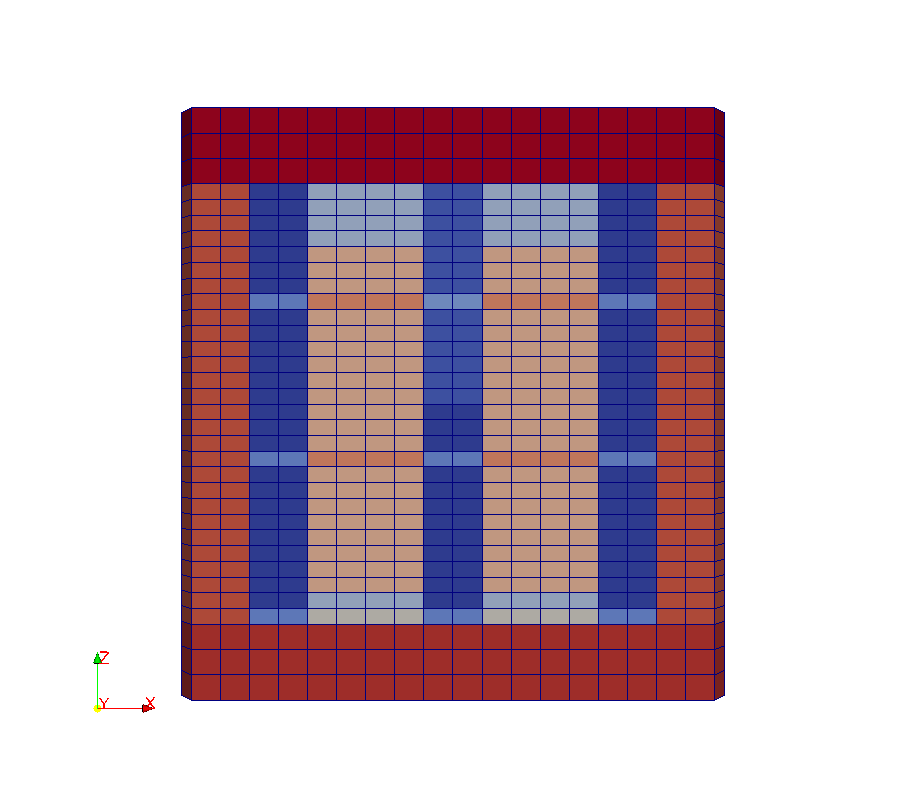
\includegraphics[scale=0.18]{carem_geom_1.png}
		%~ \caption[]{t=0 s}
		%~ \label{asd}	
	\end{minipage}
	\begin{minipage}{0.48\linewidth}
		\centering
		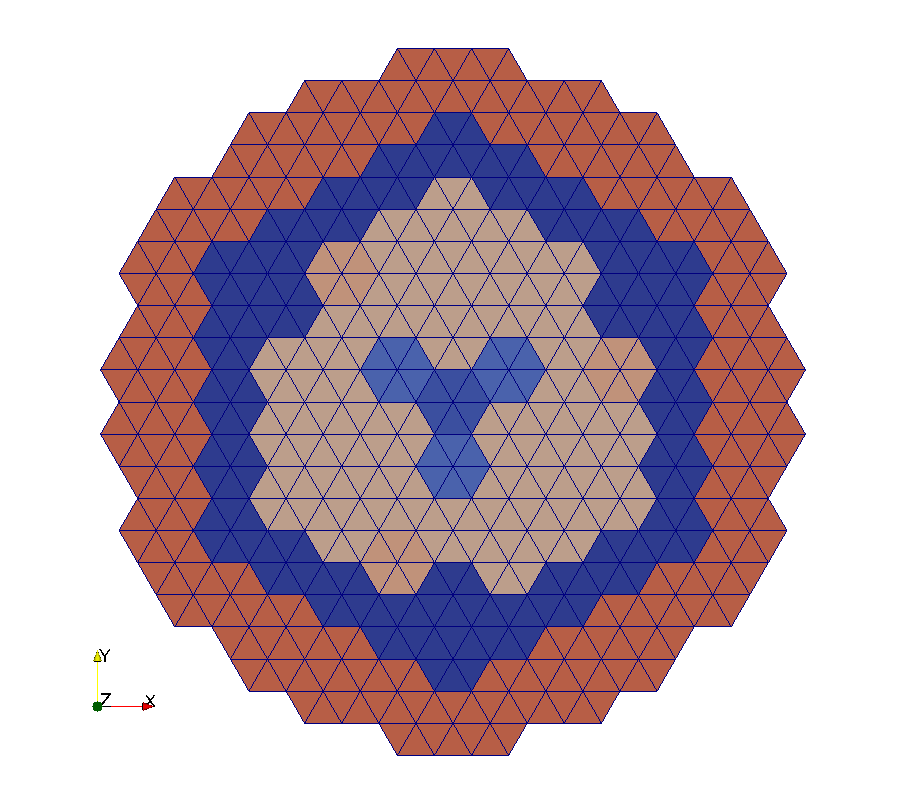
\includegraphics[scale=0.15]{carem_geom_2.png}
		%~ \caption[]{t=40 s}
		%~ \label{asd}	
	\end{minipage}
\end{figure}

\end{frame}



\scriptsize
\begin{frame}
{Ejemplos de aplicación}
{Extensión a problemas acoplados en modelos de núcleo}

Acoplamiento de \textbf{PUMA} y \textbf{RELAP5} en modelo de núcleo de CAREM-25:

\begin{figure}[ht]
	\begin{minipage}{0.48\linewidth}
      \centering
      \includegraphics[scale=0.06]{carem_burnup_10day.png}
		\caption[]{t=10 días}
		%~ \label{asd}	
	\end{minipage}
	\begin{minipage}{0.48\linewidth}
		\centering
		\includegraphics[scale=0.12]{carem_burnup_400day.png}
		\caption[]{t=400 días}
		%~ \label{asd}	
	\end{minipage}
\end{figure}
\visible<2->{

\begin{table}[h!]
  \centering
  \begin{tabular}{ c c c c c } 
      \hline
      \multicolumn{1}{c}{Método} & \multirow{1}{*}{$\Delta$t} & \multicolumn{1}{c}{Extrapolación} & \multicolumn{1}{c}{Evaluaciones} & \multicolumn{1}{c}{Tiempo} \\ % \hline
      \multicolumn{1}{c}{no lineal} & [días] & \multicolumn{1}{c}{de $\bar{x}^n$} & \multicolumn{1}{c}{totales} & \multicolumn{1}{c}{total [s]}\\ \hline %\hline
      Picard & 5 & $\mathscr{O}(0)$ & 243 & 11019 \\ %\hline
      Picard & 5 & $\mathscr{O}(1)$ & 195 & 9085  \\ %\hline
      Picard & 10 & $\mathscr{O}(0)$ & 131 & 5898 \\ %\hline            
      Picard & 10 & $\mathscr{O}(1)$ & 104 & 4774 \\ %\hline            
      Punto fijo & 5 & $\mathscr{O}(0)$ & 139 & 5415 \\ %\hline            
      Punto fijo & 5 & $\mathscr{O}(1)$ & 186 & 6990 \\ %\hline            
      Punto fijo & 10 & $\mathscr{O}(0)$ & 101 & 3755  \\ % \hline      
      Punto fijo & 10 & $\mathscr{O}(1)$ & 107 & 3919  \\ \hline            
   \end{tabular}   
   \caption[Evaluaciones totales y tiempo total requerido por cada método no lineal en cálculo de quemado con \textbf{RELAP5} y \textbf{Fermi}]
   {\scriptsize Evaluaciones totales y tiempo total requerido por cada método no lineal.}
   \label{tab-relap-puma}
\end{table}



}

\end{frame}
 % cfd
\section{Conclusiones}

\subsection*{Conclusiones I}

\begin{frame}{Conclusiones}{Conclusiones I}

\end{frame} % conclusiones
\begin{frame}[allowframebreaks]
\begin{flushright}
\huge{Gracias por su atención!}
\end{flushright}
\end{frame} % fin
% All of the following is optional and typically not needed. 
\appendix
\section<presentation>*{\appendixname}


% \subsection<presentation>*{}

% \begin{frame}[allowframebreaks]
% \begin{flushright}
% \huge{Gracias por su atención!}
% \end{flushright}
% \end{frame}



\subsection<presentation>*{For Further Reading}

\begin{frame}[allowframebreaks]
  \frametitle<presentation>{For Further Reading}
    
  \begin{thebibliography}{10}
    
  \beamertemplatebookbibitems
  % Start with overview books.

  \bibitem{Author1990}
    A.~Author.
    \newblock {\em Handbook of Everything}.
    \newblock Some Press, 1990.
 
    
  \beamertemplatearticlebibitems
  % Followed by interesting articles. Keep the list short. 

  \bibitem{Someone2000}
    S.~Someone.
    \newblock On this and that.
    \newblock {\em Journal of This and That}, 2(1):50--100,
    2000.
  \end{thebibliography}
\end{frame}

% Section and subsections will appear in the presentation overview
% and table of contents.
% \section{First Main Section}

% \subsection{First Subsection}

% \begin{frame}{First Slide Title}{Optional Subtitle}
%   \begin{itemize}
%   \item {
%     My first point.
%   }
%   \item {
%     My second point.
%   }
%   \end{itemize}
% \end{frame}

% \subsection{Second Subsection}

% % You can reveal the parts of a slide one at a time
% % with the \pause command:
% \begin{frame}{Second Slide Title}
%   \begin{itemize}
%   \item {
%     First item.
%     \pause % The slide will pause after showing the first item
%   }
%   \item {   
%     Second item.
%   }
%   % You can also specify when the content should appear
%   % by using <n->:
%   \item<3-> {
%     Third item.
%   }
%   \item<4-> {
%     Fourth item.
%   }
%   % or you can use the \uncover command to reveal general
%   % content (not just \items):
%   \item<5-> {
%     Fifth item. \uncover<6->{Extra text in the fifth item.}
%   }
%   \end{itemize}
% \end{frame}

% \section{Second Main Section}

% \subsection{Another Subsection}

% \begin{frame}{Blocks}
% \begin{block}{Block Title}
% You can also highlight sections of your presentation in a block, with it's own title
% \end{block}
% \begin{theorem}
% There are separate environments for theorems, examples, definitions and proofs.
% \end{theorem}
% \begin{example}
% Here is an example of an example block.
% \end{example}
% \end{frame}

% % Placing a * after \section means it will not show in the
% % outline or table of contents.
% \section*{Summary}

% \begin{frame}{Summary}
%   \begin{itemize}
%   \item
%     The \alert{first main message} of your talk in one or two lines.
%   \item
%     The \alert{second main message} of your talk in one or two lines.
%   \item
%     Perhaps a \alert{third message}, but not more than that.
%   \end{itemize}
  
%   \begin{itemize}
%   \item
%     Outlook
%     \begin{itemize}
%     \item
%       Something you haven't solved.
%     \item
%       Something else you haven't solved.
%     \end{itemize}
%   \end{itemize}
% \end{frame}



% % All of the following is optional and typically not needed. 
% \appendix
% \section<presentation>*{\appendixname}
% \subsection<presentation>*{For Further Reading}

% \begin{frame}[allowframebreaks]
%   \frametitle<presentation>{For Further Reading}
    
%   \begin{thebibliography}{10}
    
%   \beamertemplatebookbibitems
%   % Start with overview books.

%   \bibitem{Author1990}
%     A.~Author.
%     \newblock {\em Handbook of Everything}.
%     \newblock Some Press, 1990.
 
    
%   \beamertemplatearticlebibitems
%   % Followed by interesting articles. Keep the list short. 

%   \bibitem{Someone2000}
%     S.~Someone.
%     \newblock On this and that.
%     \newblock {\em Journal of This and That}, 2(1):50--100,
%     2000.
%   \end{thebibliography}
% \end{frame}

\end{document}


